\documentclass[10pt]{article}
\usepackage{times}

\pdfoutput=1

\usepackage{microtype}
\usepackage{graphicx}
\usepackage{subcaption}
\usepackage{booktabs}
\usepackage{multirow}

\usepackage{amsfonts,amsmath,amssymb,amsthm}

\usepackage{color}
\usepackage{algorithm}
\usepackage{algorithmic}
%\usepackage{algorithmicx}
%\usepackage{algpseudocode}
% \newcommand{\RETURN}{\STATE \textbf{return} }

\usepackage{tabu}
\usepackage{url}

\usepackage{authblk}

\usepackage{parskip}


% -----------------------------------------------------------------------
\setlength{\textwidth}{6.5in}
\setlength{\textheight}{9in}
\setlength{\oddsidemargin}{0in}
\setlength{\evensidemargin}{0in}
\setlength{\topmargin}{-0.5in}

\newlength{\defbaselineskip}
\setlength{\defbaselineskip}{\baselineskip}
\setlength{\marginparwidth}{0.8in}
% -----------------------------------------------------------------------


\usepackage{etoolbox}
\newtoggle{arxiv}
\toggletrue{arxiv}

\usepackage{mathtools}
\usepackage[dvipsnames]{xcolor}

\usepackage{tkz-euclide}

% For citations
\usepackage[numbers,sort]{natbib}
\newcommand{\yrcite}[1]{\citeyearpar{#1}}

\usepackage{hyperref}
\usepackage{cleveref}

\newlength{\myfcwidth}
\setlength{\myfcwidth}{0.8\linewidth}

\newlength{\mydiagwidth}
\setlength{\mydiagwidth}{\textwidth}

\renewcommand\Authsep{\hspace{2em}}
\renewcommand\Authand{\hspace{2em}}
\renewcommand\Authands{\hspace{2em}}

\renewcommand\Authfont{\normalfont}
\renewcommand\Affilfont{\small}


\newtheorem{theorem}{Theorem}[section]
\newtheorem{corollary}{Corollary}[theorem]
\newtheorem{lemma}[theorem]{Lemma}
\newtheorem{proposition}[theorem]{Proposition}
\newtheorem{definition}[theorem]{Definition}
\newtheorem{example}{Example}[section]

\DeclareMathOperator\acosh{acosh}
\DeclareMathOperator\asin{asin}
\DeclareMathOperator\tr{trace}

\newcommand{\R}{\mathbb{R}}

\makeatletter
\setlength{\@fptop}{0pt}
\makeatother

\begin{document}

\title{Representation Tradeoffs for Hyperbolic Embeddings}
% \author{Christopher De Sa \and Megan Leszczynski \and Jian Zhang \and Alana Marzoev \and Christopher R. Aberger \and Kunle Olukotun \and Christopher R{\'e}}

\author[$\ddagger$]{Christopher De Sa}
\author[$\dagger$]{Albert Gu}
\author[$\dagger$]{Christopher R{\'e}}
\author[$\dagger$]{Frederic Sala}
\affil[$\dagger$]{Department of Computer Science, Stanford University}
\affil[$\ddagger$]{Department of Computer Science, Cornell University\vspace{4pt}}
\affil[ ]{\footnotesize{\texttt{cdesa@cs.cornell.edu}, \texttt{albertgu@stanford.edu}, \texttt{chrismre@cs.stanford.edu},\texttt{fredsala@cs.stanford.edu}}}

\maketitle


\begin{abstract}
\begin{abstract}
There is a widely-spread claim that GANs are difficult to train, and GAN architectures in the literature are littered with empirical tricks. We provide evidence against this claim and build a modern GAN baseline in a more principled manner. First, we derive a well-behaved regularized relativistic GAN loss that addresses issues of mode dropping and non-convergence that were previously tackled via a bag of ad-hoc tricks. We analyze our loss mathematically and prove that it admits local convergence guarantees, unlike most existing relativistic losses. Second, this loss allows us to discard all ad-hoc tricks and replace outdated backbones used in common GANs with modern architectures. Using StyleGAN2 as an example, we present a roadmap of simplification and modernization that results in a new minimalist baseline---\modelName (``Re-GAN''). Despite being simple, our approach surpasses StyleGAN2 on FFHQ, ImageNet, CIFAR, and Stacked MNIST datasets, and compares favorably against state-of-the-art GANs and diffusion models.\\
Code: \href{https://www.github.com/brownvc/R3GAN}{https://www.github.com/brownvc/R3GAN}
\end{abstract}
\end{abstract}

\section{Introduction}
\label{sec:introduction}
\section{Introduction}
\label{sec:intro}


Transformers, in particular decoder-only models (e.g.\ GPT~\citep{brown2020language}, Llama~\citep{touvron2023llama}) which process input sequences in a causal fashion, are one of the main drivers of modern deep learning's success.
Numerous approaches attempt to approximate the core attention layer to address its efficiency issues~\citep{tay2022efficient}, such as scaling quadratically in sequence length during training and requiring a cache of size linear in sequence length during autoregressive generation.
In parallel, a class of alternative sequence models, structured state-space models (SSMs), have emerged with linear scaling in sequence length during training and constant state size during generation.
They show strong performance on long-range tasks (e.g. S4~\citep{gu2022efficiently}) and recently matched or beat Transformers on language modeling (e.g. Mamba \citep{gu2023mamba}) at small to moderate scale.
However, the development of SSMs have appeared disjoint from the community's collective effort to improve Transformers, such as understanding them theoretically as well as optimizing them on modern hardware.
As a result, it is more difficult to understand and experiment with SSMs compared to Transformers, and it remains challenging to train SSMs as efficiently as Transformers from both an algorithmic and systems perspective.


Our main goal is to develop a rich body of theoretical connections between structured SSMs and variants of attention.
This will allow us to transfer algorithmic and systems optimizations originally developed for Transformers to SSMs, towards the goal of building foundation models that perform better than Transformers while scaling more efficiently in sequence length.
A milestone contribution in this direction was the \textbf{Linear Attention (LA)} framework \citep{katharopoulos2020transformers},
which derived a connection between autoregressive attention and linear RNNs
by showing the equivalence between ``dual forms'' of quadratic kernelized attention and a particular linear recurrence.
This duality allows new capabilities such as the ability to have both efficient parallelizable training and efficient autoregressive inference.
In the same spirit, this paper provides multiple viewpoints connecting linear-complexity SSMs with quadratic-complexity forms to combine the strengths of SSMs and attention.%
\footnote{Technically speaking, these connections only relate to certain flavors of attention; the title of this paper is an homage to \citet{katharopoulos2020transformers} which first showed that ``Transformers are RNNs''.}

\iftoggle{arxiv}{
\begin{wrapfigure}{R}{0.48\linewidth}
  \begin{center}
    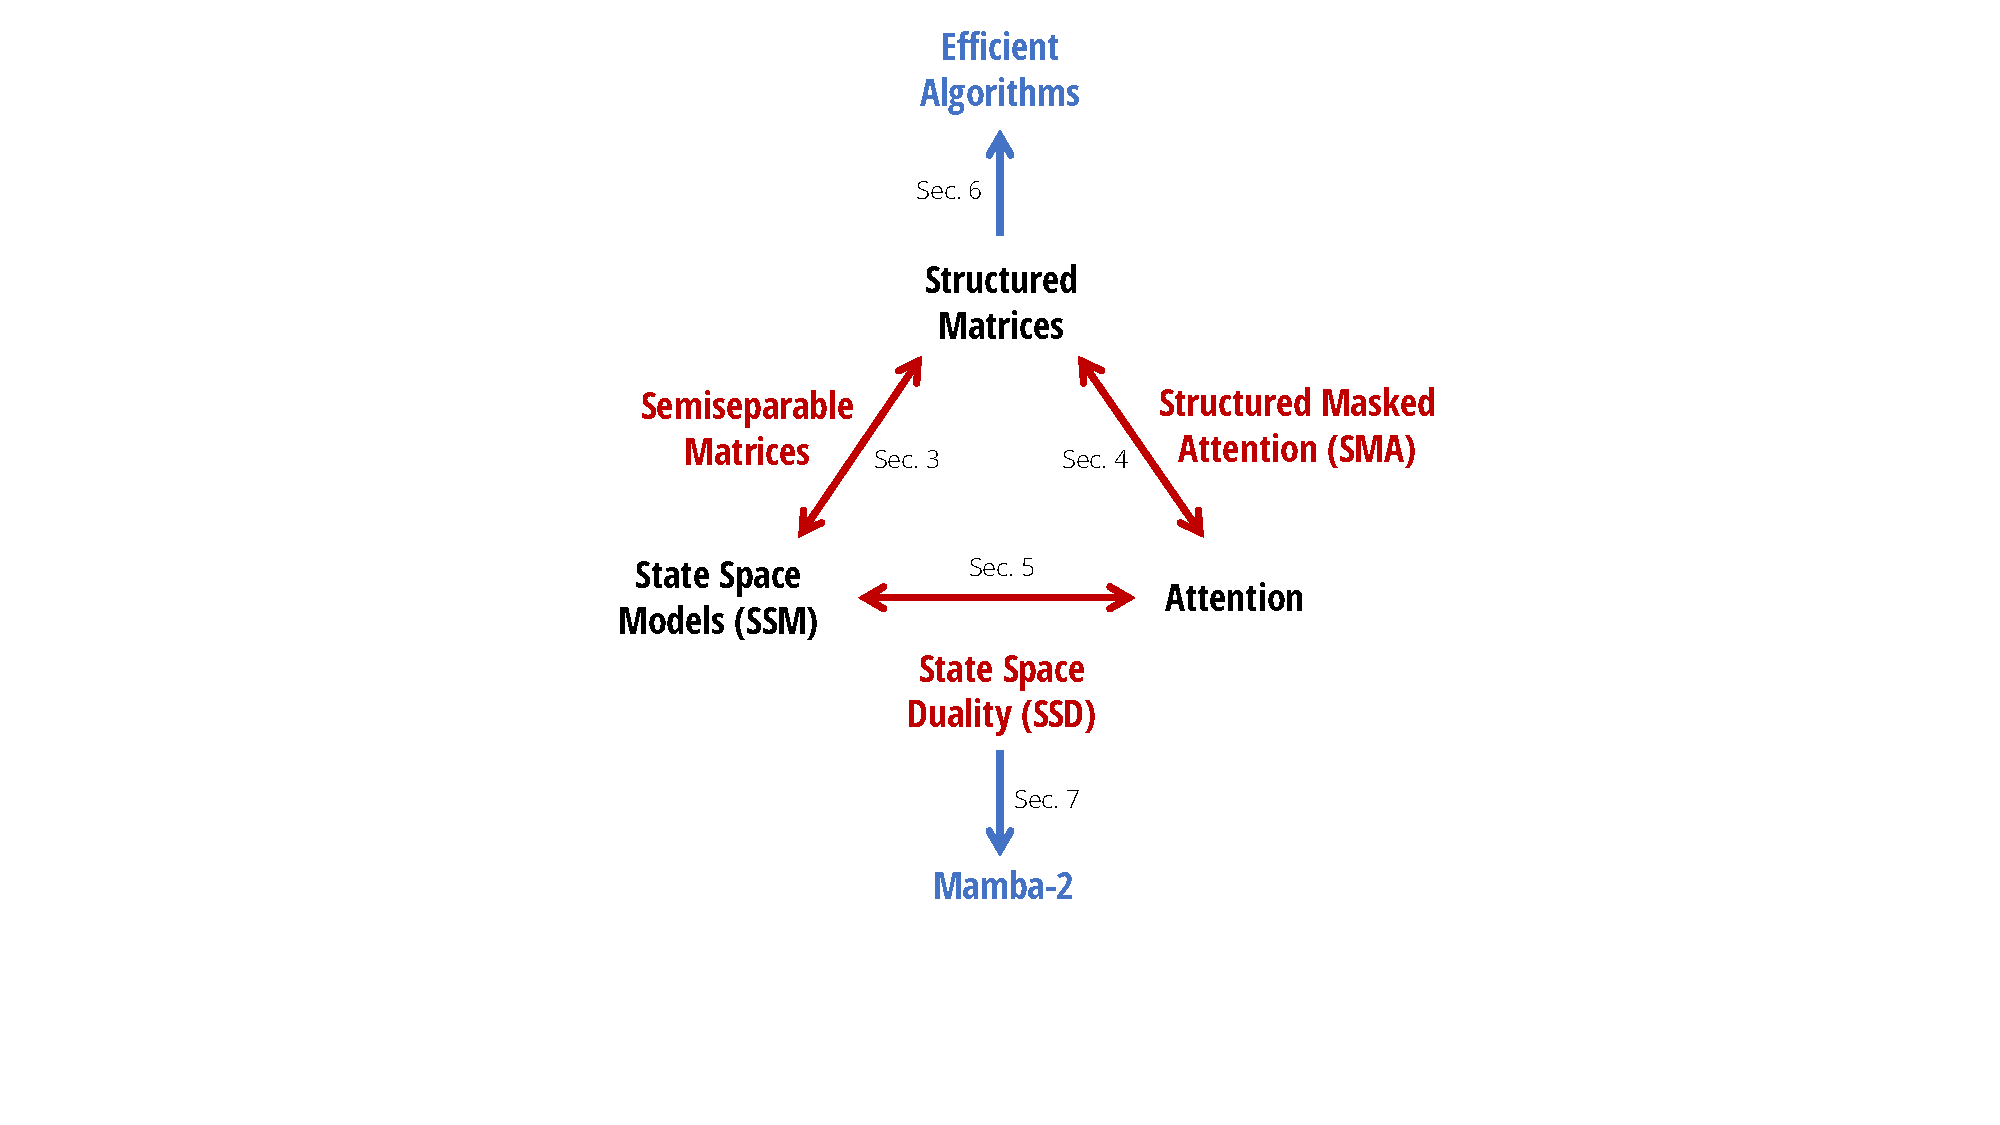
\includegraphics[width=\linewidth]{fig/ssd_roadmap.pdf}
  \end{center}
  \caption{
    (\textbf{Structured State-Space Duality}.)
    This paper fleshes out the relationship between state space models and attention through the bridge of structured matrices.
  }
  \label{fig:roadmap}
\end{wrapfigure}
}{}

\para{State Space Duality.}
Our framework connecting structured SSMs and variants of attention, which we call \textbf{structured state space duality} (SSD),
is made through the abstractions of \textbf{structured matrices}:
matrices with subquadratic parameters and multiplication complexity.
We develop two broad frameworks for representing sequence models, one as matrix transformations and one as tensor contractions, which each reveal different perspectives of the duality.
Our technical contributions include:
\begin{itemize}[leftmargin=*,itemsep=0pt,topsep=0pt]
  \item We show an equivalence between state space models and a well-studied family of structured matrices called \textbf{semiseparable matrices}\iftoggle{arxiv}{ (\cref{sec:ssm})}{}.
    This connection is at the heart our framework, revealing new properties and algorithms for SSMs. A central message of this paper is that \emph{different methods of computing state space models can be reframed as various matrix multiplication algorithms on structured matrices}.
  \item We significantly improve the theory of linear attention~\citep{katharopoulos2020transformers}.
    We first provide an incisive proof of its recurrent form through the language of tensor contractions, and then generalize it to a new family of \textbf{structured masked attention (SMA)}\iftoggle{arxiv}{ (\cref{sec:attention})}{}.
  \item We connect SSMs and SMA, showing that they have a large intersection that are duals of each other, possessing both SSM-like linear and attention-like quadratic forms\iftoggle{arxiv}{ (\cref{sec:ssd})}{}.
    \iftoggle{arxiv}{We also prove that any kernel attention method possessing a fast recurrent form must be an SSM.}{}
\end{itemize}


Beyond its intrinsic theoretical value, our framework opens up a broad set of directions for understanding and improving sequence models.

\para{Efficient Algorithms.}
First and most importantly, our framework exposes new efficient and easily-implementable algorithms for computing SSMs\iftoggle{arxiv}{ (\cref{sec:efficient})}{}.
We introduce a new \textbf{SSD algorithm}, based on block decompositions of semiseparable matrices, that takes advantage of both the linear SSM recurrence and quadratic dual form, obtaining optimal tradeoffs on all main efficiency axes (e.g. training and inference compute, memory usage, and ability to leverage matrix multiplication units on modern hardware).
A dedicated implementation of SSD is $2-8\times$ faster than the optimized selective scan implementation of Mamba, while simultaneously allowing for much larger recurrent state sizes ($8\times$ the size of Mamba or even higher, with minimal slowdown).
SSD is highly competitive with optimized implementations of softmax attention (FlashAttention-2~\citep{dao2023flashattention2}), crossing over at sequence length 2K and 6$\times$ faster at sequence length 16K.


\iftoggle{arxiv}{
\para{Architecture Design.}
One major obstacle to adopting new architectures such as SSMs is the ecosystem tailored to Transformers, such as hardware-efficient optimization and parallelism techniques for large-scale training.
Our framework allows using established conventions and techniques for attention to build a vocabulary of architecture design choices for SSMs, and further improve them (\cref{sec:architecture}).
For example, we introduce the analog of heads from multi-head attention (MHA) to SSMs.
We show that the Mamba architecture is a \textbf{multi-input SSM (MIS)} that turns out to be analogous to \textbf{multi-value attention (MVA)}, and compare other variants of Mamba with different head structures.

We also use these ideas to make slight modifications to the Mamba block, which allows tensor parallelism to be implemented (e.g. in the style of Megatron~\citep{shoeybi2019megatron}).
The main ideas include introducing grouped-value attention (GVA) head structure, and moving all data-dependent projections to occur in parallel at the beginning of the block.


}{
  \para{Mamba-2.}
  Additionally, inspired by the connection between SSMs and Transformers, we slightly modify the neural network architecture of Mamba by moving all data-dependent projections to occur in parallel at the beginning of the block. %
}
The combination of the modified parallel Mamba block, together with using SSD as the inner SSM layer, results in the \textbf{Mamba-2} architecture.
We investigate Chinchilla scaling laws for Mamba-2 in the same setting as Mamba, finding that it Pareto dominates Mamba and Transformer++ in both perplexity and wall-clock time.
We additionally train a family of Mamba-2 models at varying sizes on the Pile, showing that it matches or outperforms Mamba and open source Transformers on standard downstream evaluations.
For example, Mamba-2 with 2.7B parameters trained on 300B tokens on the Pile outperforms Mamba-2.8B, Pythia-2.8B and even Pythia-6.9B trained on the same dataset.

\iftoggle{arxiv}{
\paragraph{Systems Optimizations.}
The SSD framework connects SSMs and Transformers, allowing us to leverage a rich body of work on systems optimizations developed for Transformers~(\cref{sec:systems}).
\begin{itemize}[leftmargin=*,itemsep=0pt,topsep=0pt]
  \item For example, Tensor Parallelism (TP) is an important model parallelism technique to train large Transformer models by splitting each layer across GPUs on the same node.
    We design Mamba-2 to be TP-friendly, reducing the number of synchronization point per block by half.
  \item For very long sequences whose activations do not fit on one device, sequence parallelism has been developed for the attention blocks.
    We describe how to train SSMs in general and Mamba-2 in particular with sequence parallelism, by passing the recurrent states between devices.
  \item For finetuning with examples of different lengths, for best efficiency, Transformer requires sophisticated techniques to remove padding tokens and perform attention on variable length sequences.
    We show how Mamba-2 can be trained with variable sequence lengths efficiently, requiring no padding tokens.
\end{itemize}
}{}

\cref{sec:experiments} empirically validates Mamba-2 on language modeling, training efficiency, and a difficult multi-query associative recall task~\citep{arora2024simple}.
Finally, in \cref{sec:related}, we provide an extended related work and discuss potential research directions opened up by our framework.

Model code and pre-trained checkpoints are open-sourced at \url{https://github.com/state-spaces/mamba}.







\section{Background}
\label{sec:background}
\subsection{Data Augmentation in NLP}
The problem of domain adaptation and OOD robustness is well established in NLP \citep{blitzer-etal-2007-biographies,daume-iii-2007-frustratingly,hendrycks2020pretrained}.
Existing work on improving generalization has focused on data augmentation, where synthetically generated training examples are used to augment an existing dataset.
It is hypothesized that these examples induce robustness to local perturbations, which has been shown to be effective in semi-supervised and self-supervised settings \citep{bachman2014learning,szegedy2014intriguing, sajjadi2016regularization}.

Existing task-specific methods \citep{kafle-etal-2017-data} and word-level methods \citep{zhang2015character, xie2017data, wei-zou-2019-eda} are based on human-designed heuristics.
Back-translation from or through another language has been applied in the context of machine translation \citep{sennrich2016improving}, question answering \citep{wei2018fast}, and consistency training \citep{xie2019unsupervised}.
More recent work has used word embeddings \citep{wangyang2015thats} and LSTM language models \citep{fadaee2017data} to perform word replacement.
Other methods focus on fine-tuning contextual language models \citep{kobayashi-2018-contextual,wu2019conditional,kumar20202data} or large generative models \citep{lambada,yang2020g-daug,kumar20202data} to generate synthetic examples.

\subsection{VRM and the Manifold Assumption}
Vicinal Risk Minimization (VRM) \citep{vicinal200olivier} formalizes data augmentation as enlarging the training set support by drawing samples from a \textit{vicinity} of existing training examples.
Typically the vicinity of a training example is defined using dataset-dependent heuristics.
For example, in computer vision, examples are generated using scale augmentation \citep{simonyan2014very}, color augmentation \citep{krizhevsky2012imagenet}, and translation and rotation \citep{Simard1998}.

The \textit{manifold assumption} states that high dimensional data concentrates around a low-dimensional manifold \citep{chapelle2006semi}.
This assumption allows us to define the vicinity of a training example as its \textit{manifold neighborhood}, the portion of the neighborhood that lies on the data manifold.
Recent methods have used the manifold assumption to improve robustness by moving examples towards a decision boundary \citep{kanbak2018geometric}, generating adversarial examples \cite{szegedy2014intriguing,miyato2017virtual}, interpolating between pairs of examples \citep{zhang2018mixup}, or finding affine transforms \citep{paschali2019data}.

\begin{figure}[t!]
\centering
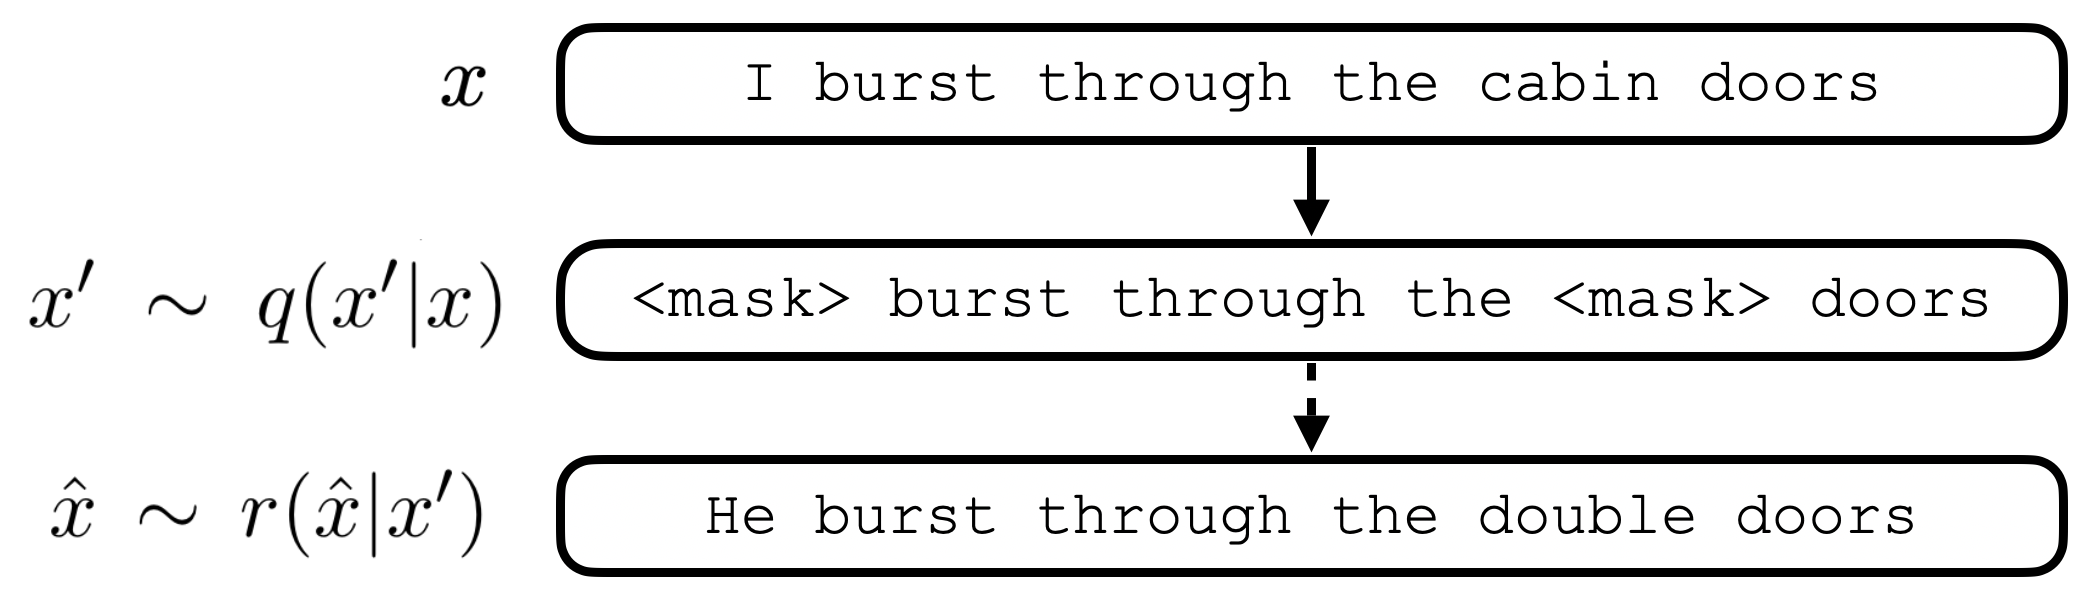
\includegraphics[scale=0.21]{img/bert_dae.png}
\caption{To sample from an MLM DAE, we apply the MLM corruption $q$ to the original sentence then reconstruct the corrupted sentence using our DAE $r$.}
\label{fig:dae_sampling}
\end{figure}

\subsection{Sampling from Denoising Autoencoders}
A denoising autoencoder (DAE) is an autoencoder trained to reconstruct a clean input $x$ from a stochastically corrupted one $x'\sim q(x'|x)$ by learning a conditional distribution $P_\theta (x| x')$ \citep{vincent2008extracting}.
We can sample from a DAE by successively corrupting and reconstructing an input using the following pseudo-Gibbs Markov chain: $x_t' \sim q(x'|x_{t-1})$, $x_t \sim P_\theta(x|x'_t).$
\comment{
\begin{align*}
    x_t' &\sim q(x'|x_{t-1})\\
    x_t &\sim P_\theta(x|x'_t) 
\end{align*}
}
As the number of training examples increases, the asymptotic distribution $\pi_n(x)$ of the generated samples approximate the true data-generating distribution $P(x)$ \citep{bengio2013generalized}.
This corruption-reconstruction process allows for sampling directly along the manifold that $P(x)$ concentrates on.

\subsection{Masked Language Models}
Recent advances in unsupervised representation learning for natural language have relied on pre-training models on a \textit{masked language modeling} (MLM) objective \citep{devlin2018, liu2019roberta}.
In the MLM objective, a percentage of the input tokens are randomly corrupted and the model is asked to reconstruct the original token given its left and right context in the corrupted sentence.
We use MLMs as DAEs \citep{lewis2019bart} to sample from the underlying natural language distribution by corrupting and reconstructing inputs (Figure \ref{fig:dae_sampling}).


\section{Combinatorial Constructions}
\label{sec:combinatorial}


%                I feel like we need some chart here to show how precision scales intuitively for folks (i.e, what’s in the experiments could come up here).

%                Hyperbolics produce low distortion and even low MAP for short bushy… also back this up with numbers from your experiments!
%                Say that the scale is critically important here. Explain that you can simply add in a learnable scale parameter. Mention a micro experiment where it has an impact, and then comment if you think it’s important more broadly.
%            Now you can devote as much as you want to the proof. 
%                You could just give the intuition of each (the precision and the lower bound).
%                I think it’s fine to say this is the key element of the proof.  
%        Embedding trees. Figure 4 is very good. 
%            You should push credit to Abraham earlier (when you mention Steiner nodes). Our contribution is applying them to these embeddings, we build on their iddeas.
%             Line 284. Probably make the is an example environment. Make sure it’s clear the reader needs to transition.
%            Make sure this section is a little more sandwich method (you don’t tell them up front—need more signposting)

We first focus on hyperbolic tree embeddings---a natural approach
considering the tree-like behavior of hyperbolic space.  We
review the embedding of \citet{sarkar} to higher dimensions. We then
provide novel analysis about the precision of the embeddings that
reveals fundamental limits of hyperbolic embeddings. In particular, we
characterize the bits of precision needed for hyperbolic
representations. We then extend the construction to $r$ dimensions,
and we propose to use Steiner nodes to better embed general graphs as
trees building on a condition from \citet{Abraham}.

\paragraph*{Embedding trees} The nature of hyperbolic space lends itself towards excellent tree embeddings. In fact, it is possible to embed trees into the Poincar\'{e} disk $\mathbb{H}_2$ with arbitrarily low distortion \cite{sarkar}. Remarkably, trees cannot be embedded into Euclidean space with arbitrarily low distortion for \emph{any} number of dimensions. These notions motivate the following two-step process for embedding hierarchies into hyperbolic space.
\begin{enumerate}
  \setlength\itemsep{0em}
\item Embed the graph $G=(V,E)$ into a tree $T$,
\item Embed $T$ into the Poincar\'{e} ball $\mathbb{H}_d$.
\end{enumerate}

We refer to this process as the \emph{combinatorial construction}. Note that we are not required to minimize a loss function. We begin by describing the second stage, where we extend an elegant construction from \citet{sarkar}. 

\subsection{Sarkar's Construction}
Algorithm~\ref{alg:sarkar} implements a simple embedding of trees into $\mathbb{H}_2$. The algorithm takes as input a scaling factor $\tau$ a node $a$ (of degree $\operatorname{deg}(a)$) from the tree with parent node $b$. Suppose $a$ and $b$ have already been embedded into $\mathbb{H}_2$ and have corresponding embedded vectors $f(a)$ and $f(b)$. The algorithm places the children $c_1, c_2, \ldots, c_{\operatorname{deg}(a)-1}$ into $\mathbb{H}_2$ through a two-step process. 

First, $f(a)$ and $f(b)$ are reflected across a geodesic (using circle inversion) so
that $f(a)$ is mapped onto the origin $0$ and $f(b)$ is mapped onto some point $z$.
% We compute the angle of $Z'$.
Next, we place the children nodes to vectors $y_1, \ldots, y_{d-1}$ equally spaced around a circle with radius $\frac{e^\tau-1}{e^\tau+1}$ (which is a circle of radius $\tau$ in the hyperbolic metric), and maximally separated from the reflected parent node embedding $z$. Lastly, we reflect all of the points back across the geodesic. 
Note that the isometric properties of reflections imply that all children are now at hyperbolic distance exactly $\tau$ from $f(a)$.

\begin{algorithm}[t]
\begin{algorithmic}[1]
\STATE \textbf{Input:} Node $a$ with parent $b$, children to place $c_1, c_2, \ldots, c_{\operatorname{deg}(a)-1}$, partial embedding $f$ containing an embedding for $a$ and $b$, scaling factor $\tau$
\STATE $(0, z) \leftarrow \operatorname{reflect}_{f(a) \rightarrow 0}(f(a),f(b))$ %\COMMENT{circle inversion}
\STATE $\theta \leftarrow \operatorname{arg}(z)$ \hspace{2em} \COMMENT{angle of $z$ from x-axis in the plane}
\FOR{$i \in \{1, \ldots, \operatorname{deg}(a)-1 \}$}
\STATE $y_i \leftarrow \left(\frac{e^\tau-1}{e^\tau+1} \cdot \cos\left(\theta + \frac{2\pi i}{\operatorname{deg}(a)} \right) , \frac{e^\tau-1}{e^\tau+1} \cdot \sin\left(\theta+\frac{2\pi i}{\operatorname{deg}(a)}\right) \right)$ % \label{alg:sarkar:step:circle}
\ENDFOR
\STATE $(f(a), f(b), f(c_1),\ldots,f(c_{\operatorname{deg}(a)-1})) \leftarrow \operatorname{reflect}_{0 \rightarrow f(a)}(0, z, y_1, \ldots, y_{\operatorname{deg}(x)-1})$
\STATE \textbf{Output:} Embedded $\mathbb{H}_2$ vectors $f(c_1), f(c_2), \ldots, f(c_{\operatorname{deg}(a)-1})$
\end{algorithmic}
\caption{Sarkar's Construction}
\label{alg:sarkar}
\end{algorithm}

To embed the entire tree, we place the root at the origin $O$ and its children in a circle around it (as in Step~5 of Algorithm~\ref{alg:sarkar}), then recursively place their children until all nodes have been placed. Notice this construction runs in linear time.

\subsection{Analyzing Sarkar's Construction}
\label{sec:sarkar}
The \emph{Voronoi cell} around a node $a \in T$ consists of points $x \in \mathbb{H}_2$ such that $d_H(f(a),x) \leq d_H(f(b),x)$ for all $b \in T$ distinct from $a$. That is, the cell around $a$ includes all points closer to $f(a)$ than to any other embedded node of the tree. Sarkar's construction produces Delauney embeddings: embeddings where the Voronoi cells for points $a$ and $b$ touch only if $a$ and $b$ are neighbors in $T$. Thus this embedding will preserve neighborhoods.

A key technical idea exploited by \citet{sarkar} is to scale all the
edges by a factor $\tau$ before embedding. We can then recover the original distances
by dividing by $\tau$. This transformation exploits the fact that
hyperbolic space is not {\em scale invariant}.
Sarkar's construction always captures neighbors perfectly, but Figure~\ref{fig:geod} implies that increasing the scale preserves the distances between farther nodes better.
Indeed, if one sets
$\tau
= \frac{1+\varepsilon}{\varepsilon}\left(2\log \frac{\operatorname{deg}_{\max}}{\pi
/2}\right)$, then the worst-case distortion $D$ of the resulting embedding is no more than
$1+\varepsilon$. For trees, Sarkar's construction has arbitrarily high
fidelity. However, this comes at a cost: the scaling $\tau$ affects
the bits of precision required. In fact, we will show that the
precision scales logarithmically with the degree of the tree---but linearly with the maximum path length. We use
this to better understand the situations in which hyperbolic
embeddings obtain high quality.

%Algorithm~\ref{alg:sarkar} produces edges scaled by $\nu$. That is, a unit distance has been scaled to $\nu$, and we can recover the original distances by dividing by $\nu$. Choosing $\nu$ correctly allows us to bound the distortion $d_{wc}$ of the embedding to $1+\varepsilon$ for any $\varepsilon > 0$.


%We call this Sarkar's condition.

%We build on the $\mathbb{H}_2$ construction from \citet{sarkar}. This approach produces Delauney embeddings, i.e., embeddings $f$ where the Voronoi cells for points $f(x),f(y)$ \footnote{The \emph{Voronoi cell} around $f(x)$ consists of points $\alpha \in \mathbb{H}_2$ such that $d_H(f(x),\alpha) \leq d_H(f(y),\alpha)$ for all $y \in T$ distinct from $x$. That is, the cell around $f(x)$ includes all points closer to $f(x)$ than any other embedded vertex of the tree.} touch only if $x,y$ are neighbors in $T$. The basic idea is to embed the children of $x$ so that each child is placed inside a disjoint cone emanating from $x$. Moreover, the cones rooted at child $y$ lie inside the cone rooted at $x$ containing $y$, so that Voronoi cells around nodes in different subtrees cannot touch. Full details on this approach are found in \citet{sarkar}.

How many bits of precision do we need to represent points in
$\mathbb{H}_2$? If $x \in \mathbb{H}_2$, then $\|x \| < 1$, so we need
sufficiently many bits so that $1 - \|x\|$ will not be rounded to zero. This requires
roughly $-\log (1-\|x\|) = \log \frac{1}{1-\|x\|}$ bits.  Say we are
embedding two points $x,y$ at distance $d$. As described in the
background, there is an isometric reflection that takes a pair of points $(x,y)$
in $\mathbb{H}_2$ to $(0,z)$ while preserving their distance, so
without loss of generality we have that
\[ d = d_H(x, y) = d_H(0,z) = \acosh \left(1+2\frac{\|z\|^2}{1-\|z\|^2} \right). \]
Rearranging the terms, we have \[\frac{\cosh(d)+1}{2} = \frac{1}{1-\|z\|^2} \ge \frac{1/2}{1-\|z\|}.\] Thus, the number of bits we want so that $1 - \|z\|$ will not be rounded to zero is $\log ( \cosh(d)+1)$. Since $\cosh(d) = (\exp(d)+\exp(-d))/2$, this is roughly $d$ bits.
That is, in hyperbolic space, we need about $d$ bits to express distances of $d$ (rather than $\log d$ as we would in Euclidean space).%
\footnote{Although it is particularly easy to bound precision in the Poincar{\'e} model, this fact holds generally for hyperbolic space independent of model. See Appendix~\ref{app:CombinatorialProofs} for a general lower bound argument.}
This result will be of use below.

Now we consider the largest distance in the embeddings produced by Algorithm~\ref{alg:sarkar}. If the longest path in the tree is $\ell$, and each edge has length $\tau = \frac{1}{\varepsilon}\left(2\log \frac{\operatorname{deg}_{\text{max}}}{\pi /2}\right)$, the largest distance is $O(\frac{\ell}{\varepsilon}\log \operatorname{deg}_{\text{max}})$, and we require this number of bits for the representation.

We interpret this expression. Note that $\operatorname{deg}_{\max}$ is inside the $\log$ term, so that a bushy tree is not penalized much in precision. On the other hand, the longest path length $\ell$ is not, so that hyperbolic embeddings struggle with long paths. 
Moreover, by selecting an explicit graph, we derive a matching lower
bound, concluding that to achieve a distortion $\varepsilon$, any
construction requires $\Omega\left(\frac{\ell}{\varepsilon} \log (\text{deg}_{\max}) \right)$
bits, which matches the upper bound of the combinatorial
construction. The argument follows from selecting a graph consisting
of $m(\text{deg}_{\max}+1)$ nodes in a tree with a single root and $\text{deg}_{\max}$ chains each of length $m$. The
proof of this result is described in Appendix~\ref{app:CombinatorialProofs}.

%% \begin{figure}
%% \centering
%% 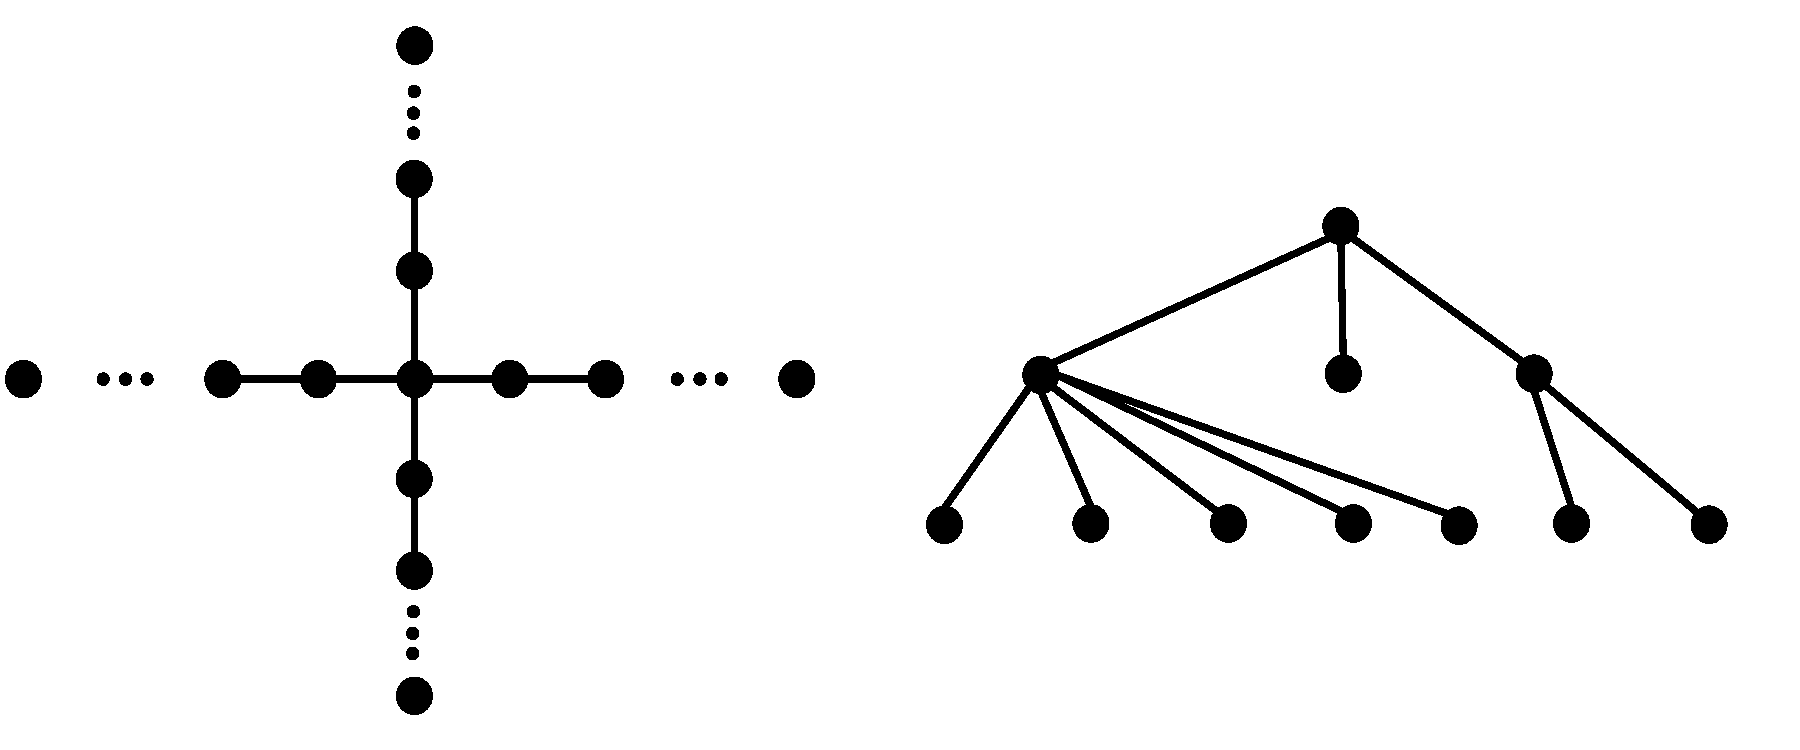
\includegraphics[width=0.50\textwidth]{figures/chain2.pdf}
%% \caption{Graphs with long chains are difficult for hyperbolic embeddings (left) while short bushy trees are easy (right).}
%% \label{fig:chains}
%% \end{figure}

%Our implementation of the construction follows \cite{Sarkar} closely, with simple modifications required by the fact that in \cite{Sarkar}, the construction is performed in (abstract) hyperbolic space, while we work with the Poincar\'{e} models. 

\subsection{Improving the Construction}



%\begin{table}[tb]
%\centering
%\begin{tabular}{|l||c|c|c|c|c|}
%\hline 
%Dataset & Nodes & $d_{\max}$ &  $r=2$ & $r=3$ & $r=5$ \\    \hline    \hline
%Bal. Tree     & 40    &4  & 25 & 13  & 13 \\ \hline
%Phy. Tree & 344  &16 & 425 & 142 & 107\\ \hline
%\end{tabular}
%\caption{Precision upper bound required for combinatorial construction at $\varepsilon=1.0$ tolerance for two trees described in Section~\ref{sec:experiments}.}
%\label{table:bitcost}
%\end{table}

Our next contribution is a generalization of the construction from the disk $\mathbb{H}_2$ to the ball $\mathbb{H}_r$. Our construction follows the same line as Algorithm~\ref{alg:sarkar}, but since we have $r$ dimensions, the step where we place children spaced out on a circle around their parent now uses a hypersphere.

Spacing out points on the hypersphere is a classic problem known as \emph{spherical coding} \cite{Spheres}. As we shall see, the number of children that we can place for a particular angle grows with the dimension. Since the required scaling factor $\tau$ gets larger as the angle decreases, we can reduce $\tau$ for a particular embedding by increasing the dimension. Note that increasing the dimension helps with bushy trees (large $\operatorname{deg}_{\max}$), but has limited effect on tall trees with small $\operatorname{deg}_{\max}$. We show

%there are $r-1$ angles $\theta_1, \ldots, \theta_{r-1}$. We divide the angles into $k$ parts, allowing us to place $\Theta(k^{r-1})$ children around any node for $k\geq 2$. Since we need $k^{r-1} \geq \operatorname{deg}_{\max}$, we can ultimately reduce the precision linearly in $r$ for $r$ up to $\leq (\log \operatorname{deg}_{\max})+1$. 


\begin{proposition} The generalized $\mathbb{H}_r$ combinatorial construction has distortion at most $1+\varepsilon$ and requires at most $O(\frac{1}{\varepsilon}\frac{\ell}{r} \log \operatorname{deg}_{\max})$ bits to represent a node component for $r \leq (\log \operatorname{deg}_{\max})+1$, and $O(\frac{1 }{\varepsilon}\ell)$ bits for $r > (\log \operatorname{deg}_{\max})+1$. 
\end{proposition}

The algorithm for the generalized $\mathbb{H}_r$ combinatorial construction replaces Step~5 in Algorithm~\ref{alg:sarkar} with a node placement step based on ideas from coding theory. The children are placed at the vertices of a hypercube inscribed into the unit hypersphere (and afterwards scaled by $\tau$). Each component of a hypercube vertex has the form $\frac{\pm 1}{\sqrt{r}}$. We index these points using binary sequences ${a} \in \{0,1\}^r$ in the following way:

\[{x}_{ a} = \left( \frac{(-1)^{a_1}}{\sqrt{r}}, \frac{(-1)^{a_2}}{\sqrt{r}} , \ldots, \frac{(-1)^{a_r}}{\sqrt{r}} \right).\]

We can space out the children by controlling the distances between the children. This is done in turn by selecting a set of binary sequences with a prescribed minimum Hamming distance---a binary error-correcting code---and placing the children at the resulting hypercube vertices. We provide more details on this technique and our choice of code in the appendix.
%\begin{proof}
%Our argument connects the required edge lengths for Sarkar's condition to be met, and the number of children we can place around a node $k^{r-1}$. We require $k^{r-1} \geq d_{\max}$.

%First, we can simplify our analysis by isometrically reflecting hyperbolic space so that the parent $x$ is the origin $0$. Let this isometry take $y$ to $p$. Then, using the hyperbolic distance formula, \begin{align*} d_H&(x,y) = d_{H}(0,q) = \\ &\mathsf{acosh}\left(1 + \frac{\cos^2 \theta/2}{1 - \cos^2 \theta/2}\right) = 
 % \mathsf{acosh}\left(1 + \cot \frac{\theta}{2}\right).\end{align*}
%Now we estimate $\exp\{ d_H(x,y) \} - 1 =  \cot \frac{\theta}{2}$ yielding $\tan \frac{\theta}{2} \leq \exp\{ - d_H(x,y) \}.$

%We place rays spaced at intervals of $\pi/k$ emanating from a point in each dimension. The cones are placed aligned with these rays. The resulting lattice can thus hold $k^{r-1}$ cones. In order to place all the children of each node, we must have $k^{r-1} \geq d_{\max}$. 
%Then, the edge lengths satisfy
%\begin{align*}
%-\log &\tan \frac{\pi}{2k} = - \log \tan \frac{\pi d_{\max}^{-1/r}}{2} \approx - \log \frac{\pi d_{\max}^{-1/r}}{2} \\
%&=  \frac{1}{r} \log d_{\max} - \log \frac{\pi}{2}.
%    \end{align*}
%We only need to meet Sarkar's condition, which offers $1+\varepsilon$ distortion if each length is scaled by the former quantity times $\frac{1+\varepsilon}{\varepsilon}$. Thus we meet our distortion bound. Next, recall that for a node component, the representation requires no more bits than the maximum path length $\ell$ times the edge length for our tree; this quantity is given by 
%\begin{equation}
%O\left(\frac{1 +  \varepsilon}{\varepsilon}\frac{\ell}{r} \log d_{\max} \right),
%\label{eq:prec}
%\end{equation}
%as desired.
%\end{proof}. 

%Observe that the precision has now been decreased by a factor of $r$, the dimension.

%To gain intuition about the precision-dimension tradeoff,
%Table~\ref{table:bitcost} shows the precision bound as the embedding dimension changes for two trees.
% The key takeaways of our analysis are:
% \begin{itemize}
%   \setlength\itemsep{0em}

% \item
% There is a fundamental tension between precision and quality in
% hyperbolic embeddings.

% \item Hyperbolic embeddings have an exponential advantage in space compared to Euclidean embeddings for short, bushy hierarchies, but will have less of an advantage
% for graphs that contain long paths.

% \item Choosing an appropriate scaling factor $\tau$ is critical for quality.
% Later, we will propose to learn this scale factor automatically for computing embeddings in PyTorch.
% \end{itemize}




\subsection{Embedding into Trees}
%Since embedding trees into the Poincar\'{e} can be performed with distortion as low as we desire, it remains to consider the distortion in the first stage. 
\begin{figure}
\centering
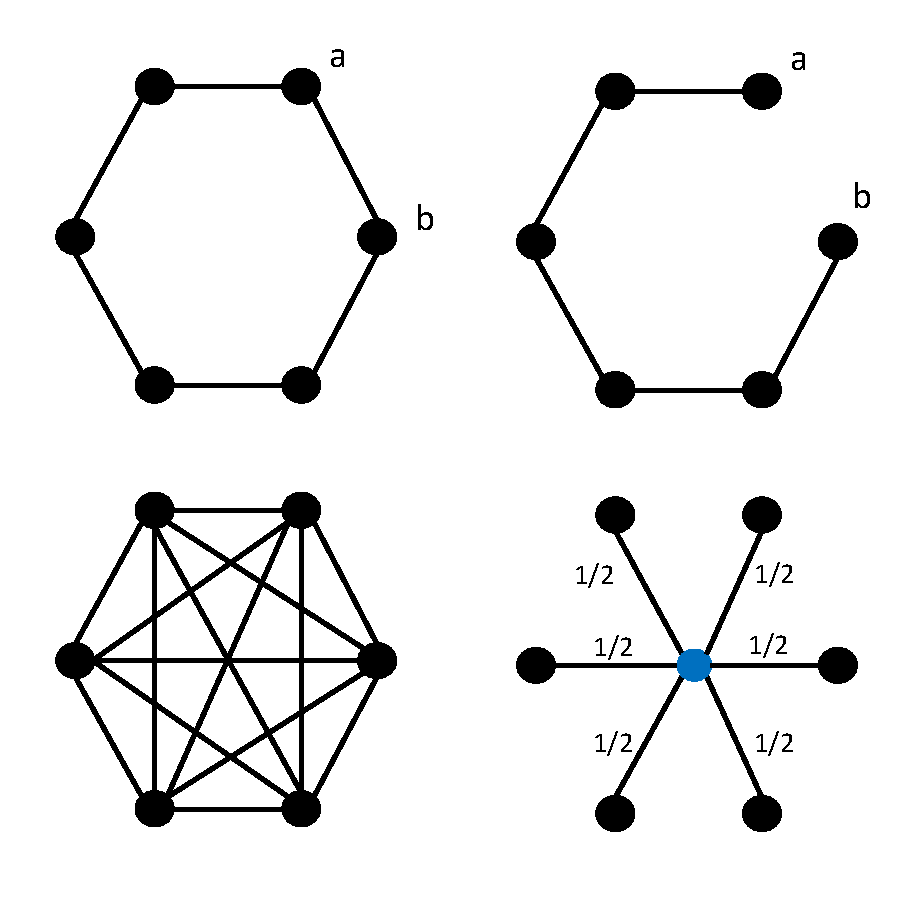
\includegraphics[width=0.3\textwidth]{figures/steiner.pdf}
\caption{Top. Cycles are a challenge for tree embeddings: $d_G(a,b)$ goes from $1$ to $5$. Bottom. Steiner nodes can help: adding a node (blue) and weighting edges maintains the pairwise distances.}
\label{fig:steiner}
\end{figure}
We revisit the first step of the construction: embedding graphs into
trees. There are fundamental limits to how well graphs can be embedded
into trees; in general, breaking long cycles inevitably adds
distortion, as shown in Figure~\ref{fig:steiner}. We are inspired by a
measure of this limit, the \emph{$\delta$-4 points condition} introduced
in \citet{Abraham}. A graph on $n$ nodes that satisfies the $\delta$-4
points condition has distortion at most $(1+\delta)^{c_1 \log n}$ for
some constant $c_1$. This result enables our end-to-end embedding to
achieve a distortion of at most \[D(f) \leq (1+\delta)^{c_1 \log n}(1
+ \varepsilon).\]

The result in \citet{Abraham} builds a tree with \emph{Steiner} nodes. These additional nodes can help control the distances in the resulting tree.
\begin{example} \label{ex:steiner}
Embed a complete graph on $\{1,2,\ldots, n\}$ into a tree. The tree will have a central node, say 1, w.l.o.g., connected to every other node; the shortest paths between pairs of nodes in $\{2,\ldots,n\}$ go from distance 1 in the graph to distance 2 in the tree. However, we can introduce a Steiner node $n+1$ and connect it to all of the nodes, with edge weights of $\frac{1}{2}$. This is shown in Figure~\ref{fig:steiner}. The distance between any pair of nodes in $\{1,\ldots,n\}$ remains 1.\end{example}

Note that introducing Steiner nodes can produce a weighted tree, but Algorithm~\ref{alg:sarkar} readily extends to the case of weighted trees by modifying Step~5.
We propose using the Steiner tree algorithm in \citet{Abraham} (used to achieve the distortion bound) for real embeddings, and we rely on it for our experiments in Section~\ref{sec:experiments}. In summary, 
the key takeaways of our analysis in this section are:
\begin{itemize}
%\setlength\itemsep{0em}
\item
There is a fundamental tension between precision and quality in
hyperbolic embeddings.

\item Hyperbolic embeddings have an exponential advantage in space compared to Euclidean embeddings for short, bushy hierarchies, but will have less of an advantage
for graphs that contain long paths.

\item Choosing an appropriate scaling factor $\tau$ is critical for quality.
Later, we will propose to learn this scale factor automatically for computing embeddings in PyTorch.
\item Steiner nodes can help improve embeddings of graphs.
\end{itemize}
%We discuss the limiting factors, mitigating these with Steiner nodes, and suitable algorithms with distortion guarantees.


%What prevents us from embedding a general graph into a tree with low distortion? The answer is long cycles. Such cycles must be broken, and the distances between the nodes adjacent to the broken edge ($a$ and $b$ in Figure~\ref{fig:steiner}) are inevitably large. Tree embeddings are therefore limited by the structure of the graph. 

%However, we can tackle this challenge by introducing \emph{Steiner} nodes, as in \citet{Abraham}. These additional nodes can help control the distances in the resulting tree:
%\begin{example} \label{ex:steiner}
%We embed a complete graph on $\{1,2,\ldots, n\}$ into a tree. The resulting tree will have a central node, say 1 w.l.o.g., connected to every other node; the shortest paths between pairs of nodes in $\{2,\ldots,n\}$ go from distance 1 in the graph to distance 2 in the tree. However, we can instead introduce a Steiner node $(n+1)$ and connect it to all of the nodes, setting edge weights of $\frac{1}{2}$. This is shown in Figure~\ref{fig:steiner}. The distance between any pair of nodes in $\{1,\ldots,n\}$ remains 1.\end{example}

%This simple example reveals the power of Steiner nodes for tree embeddings. In fact, there exist fundamental quantities measuring the best-possible tree embedding, and the algorithms that achieve these best embeddings rely on Steiner nodes. For example, the $\delta$-4 points condition is such a measure \cite{Abraham}. A graph on $n$ nodes that satisfies the $\delta$-4 points condition has distortion at most $(1+\delta)^{c_1 \log n}$ for some constant $c_1$. Since worst-case distortion is multiplicative, this enables our end-end embedding to achieve a distortion of at most  \[D \leq (1+\delta)^{c_1 \log n}(1 + \varepsilon).\]

%In other words, we have an upper bound on our overall distortion as a function of an intrinsic graph property ($\delta$) and a parameter we control ($\varepsilon$). We propose using the Steiner tree algorithm in \cite{Abraham} (used to achieve the distortion bound) for real embeddings, and we relied on it for our experiments in Section~\ref{sec:experiments}. In summary, 
%\begin{itemize}
%\item Even in general settings, consider introducing additional nodes to improve embedding quality.
%\end{itemize}
%More generally, additional nodes can improve the quality of the embedding.

%\begin{tcolorbox}
%{\bf Takeaway}: Even in general settings, we may wish to introduce extra nodes to improve embedding quality.
%\end{tcolorbox}


%There are a number of available bounds describing the distortion incurred by embedding arbitrary $n$-point metric spaces into trees \cite{Fakcharoenphol,Elkin}. However, we are particularly interested in embedding hierarchies; such graphs should offer structure that is close to tree-like. We seek a measure of tree-ness that is intrinsic to metric space and characterizes the distortion.

%There are a number of options. We rely on the $\varepsilon$-4-points condition introduced in \cite{Abraham}, where trees always achieve $\varepsilon=0$. The results in \cite{Abraham} show that a metric space $V$ on $n$ points that satisfies the $\varepsilon$-4PC for some $\varepsilon \in [0,1]$ can be embedded into a tree metric with distortion at most $(1+\varepsilon)^{c_1 \log n}$ for some constant $c_1$. Since worst-case distortion is multiplicative, the overall distortion is bounded as \[D \leq (1+\varepsilon)^{c_1 \log n}(1 + \varepsilon').\] Here we observe that $n$ and $\varepsilon$ are features of the graph, while $\varepsilon'$, the parameter controlling the hyperbolic embedding fidelity is under our control, at the cost of increasing the number of bits of precision.

%The work in \cite{Abraham} includes an algorithm that builds a Steiner tree matching the bound of $(1+\varepsilon)^{c_1 \log n}$. We implement this algorithm for the experiments detailed in Section~\ref{sec:experiments}. However, the algorithm requires $O(n^3)$ time to build a tree for $n$ points. Thus, we often opt for a simpler approach. As we shall see in our experiments, we have observed that even a simple BFS tree can be used as the embedding of choice, offering good results at a very cheap computational cost. 

%Consider four points $w,x,y,z$ in metric space $V$ ordered so that the three distance matchings $d(w,x)+d(y,z)$, $d(w,y)+d(x,z)$, $d(w,z)+d(x,y)$ satisfy $d(w,x) + d(y,z) \leq d(w,y) + d(x,z) \leq d(w,z) + d(x,y)$. Then, $V$ satisfies the $\varepsilon$-4-points condition if
%\[d(w,z) + d(x,y) \leq d(w,y) + d(x,z) + 2\varepsilon \min\{d(w,x),d(y,z)\}.\]
%That is, $\varepsilon$ measures the difference in the largest matchings, normalized by the smallest distance. Note that $\varepsilon=1$ is satisfied in all spaces $V$ by the triangle inequality. At the other extreme, if $\varepsilon=0$, the two largest distance matchings are equal and the $\varepsilon$-4PC reduces to the classical 4-points-condition \cite{Buneman}, which every tree satisfies. In other words, the $\varepsilon$ parameter reflects how tree-like the metric space $V$ is. Moreover, as shown in \cite{Abraham}, a metric space $V$ on $n$ points that satisfies the $\varepsilon$-4PC for some $\varepsilon \in [0,1]$ can be embedded into a tree metric with distortion at most $(1+\varepsilon)^{c_1 \log n}$ for some constant $c_1$.










%%%%%%%%%%%%%

%Since worst-case distortion is multiplicative, the overall distortion is bounded as \[D \leq (1+\varepsilon)^{c_1 \log n}(1 + \delta).\] Here we observe that $n$ and $\varepsilon$ are features of the graph, while $\delta$ is a parameter that we may decrease, at the cost of increasing the number of bits of precision.
% move this to appendix:
%
%\begin{proof}
%We start with the $n=1$ case. Consider any two leaf nodes
%$x,y$. First, we show that all of the leaves have equal norm, or otherwise we could equalize this distance without increasing the distortion. To see this, let the longest edge have length $b$ and the shortest have length $a$. The longest path has length at most $2a$, while the shortest path has length at least $b$. The worst-case distortion is the largest expansion (at most $2a/2 = a/1$) multiplied by the largest contraction (at worst $2/(2b)=1/b$, or $a/b$. Thus, equalizing $a/b$ can only decrease the distortion.
%
%Let $u=\|x\|$ and $\bar u = \frac{u^2}{1-u^2}$. Then, $d_{h}(0,x) =
%\mathsf{acosh}\left(1 + 2 \bar u\right)$. We then want to show that
%$\bar u = \Omega\left(\varepsilon^{-1}\right)$.
%
%We argue by considering the distance between $x$ and $y$:
%\begin{align*}
%  d_{H}(x,y) = & \mathsf{acosh}\left( 1 + 2\frac{\|x - y\|^2}{(1-\|x\|^2)(1-\|y\|^2)} \right) \\
%  = &
%  \mathsf{acosh}\left( 1 + 4(1 - \hat{x}^T\hat{y})\frac{u^2}{(1-u^2)^2} \right)
%\end{align*}
%in which $\hat{x}u = x$ and $\hat{y}u = y$.
%
%Now, since $d_{H}(x,y) \leq d_{H}(0,x) + d_{h}(0,y) = 2d_{H}(0,x)$ to achieve distortion $\varepsilon$ we must show
%\[ d_{H}(x,y) \geq 2d_{H}(0,x)(1-\varepsilon). \]
%
%We show that $\bar u =
%\Omega(\varepsilon^{-1})$, which implies we need
%$\log(\varepsilon^{-1})$ bits to represent this value, completing the $n=1$ case.
%
%Note that $\cosh$ is monotonic, so that w can write
%\begin{align*} 
%4(1 - \hat{x}^T&\hat{y})\frac{u^2}{(1-u^2)^2}\\
%& \geq \cosh(2d_{H}(0,x)(1-\varepsilon)) - 1 \\
%& =2 \left(\cosh^2(d_{H}(0,x)(1-\varepsilon)) -  1\right)
%\end{align*}
%
%
%Here, we use the estimate that
%\[ \cosh^2(z(1-\varepsilon)) \geq (1 - 2\varepsilon \cosh(z)) \cosh^{2}(z)  \]
%Next, we can write, supposing that $\hat{x}^T\hat{y} \geq 0$
%with $z=\mathrm{acosh}(1 + 2\bar u)$,
%\[ 1 + 2\frac{\bar u^2}{u^2} \geq  (1 - 2 \varepsilon (1 + 2 \bar u) )\left(1 + 2 \bar u\right)^2  \]
%\[ 0 = 2\bar u^2 {\bar u}^{-1} - 2 \bar u \geq 2 \bar u^2  + 2 \bar u- 2 \varepsilon  \left(1 + 2 \bar u\right)^3\]
%
%Now, $\frac{1}{u^2} - 1 = \frac{1 - u^2}{u^2} = \bar u^{-1}$. In turn, $\varepsilon  \geq \frac{\bar u^2 + \bar u}{(1 + 2\bar u)^3}$, that is, $\varepsilon^{-1} \leq 8 \bar u + o(\bar u)$, and we are done.
%
%Next, we consider $n>1$. Observe that $d_{H}(nx,ny) = \Omega\left( \varepsilon^{-1} n\right)$ by a similar argument. {\color{red} more details}.
%\[ d(0,x) = n\varepsilon^{-1} \implies 1 + 2 \frac{\|x\|^2}{1 - \|x\|^2} \geq \exp( n \varepsilon^{-1} ) \]
%
%Thus, we need $\Omega(n \varepsilon^{-1})$ bits to represent these
%numbers. %Note, that in general to support a dynamic range of {\em hyperbolic distances $d$}, we need $\Omega(d)$ bits.
%\end{proof}





\section{Hyperbolic Multidimensional Scaling}
\label{sec:MDS}
In this section, we explore a fundamental and more general question than we did in the previous section: if we are given the pairwise distances arising from a set of points in hyperbolic space, can we recover the points? The equivalent problem for Euclidean distances is solved with multidimensional scaling (MDS). The goal of this section is to analyze the \emph{hyperbolic MDS} (h-MDS) problem. We describe and overcome the additional technical challenges imposed by hyperbolic distances, and show that exact recovery is possible and interpretable.
Afterwards we propose a technique for dimensionality reduction using principal geodesics analysis (PGA) that provides optimization guarantees.
In particular, this addresses the shortcomings of h-MDS when recovering points that do not exactly lie on a hyperbolic manifold.
%proceed to analyze perturbations for h-MDS (i.e., recovery from noisy distances), mirroring the analysis of MDS robustness.

\subsection{Exact Hyperbolic MDS}
\label{sec:exactmds}


Suppose that there is a set of
hyperbolic points $x_1,\dots, x_n \in \mathbb{H}_r$, embedded in the Poincar{\'e} ball and written $X \in
\mathbb{R}^{n \times r}$ in matrix form.
We observe all the pairwise distances $d_{i,j} = d_H(x_i, x_j)$, but do not observe $X$:
our goal is use the observed $d_{i,j}$'s to recover $X$ (or some other set of points with the same pairwise distances $d_{i,j}$).

The MDS algorithm in the Euclidean setting makes an important
\emph{centering}%
\footnote{We say that points are centered at a particular mean
  if this mean is at $0$. The act of centering refers to applying an isometry
  that makes the mean of the points $0$.}
assumption.
That is it assumes the points have mean $0$, and it turns out that if an exact
embedding for the distances exists, it can be recovered from a matrix factorization.
In other words, Euclidean MDS always recovers a centered embedding.

In hyperbolic space, the same algorithm does not work, but we show that it is possible to find an embedding centered at a different mean. 
More precisely, we introduce a new mean which we call the \emph{pseudo-Euclidean mean}, that behaves like the Euclidean mean in that it enables recovery through matrix factorization.
Once the points are recovered in hyperbolic space, they can be recentered around a more canonical mean by translating it to the origin.

Algorithm~\ref{alg:new_hmds} is our complete algorithm, and for the remainder of
this section we will describe how and why it works.
We first describe the \emph{hyperboloid model}, an alternate but equivalent model of hyperbolic geometry in which h-MDS is simpler. Of course, we can easily convert between the hyperboloid model and the Poincar\'{e} ball model we have used thus far.
Next, we show how to reduce the problem to a standard PCA problem, which recovers an embedding centered at the points' pseudo-Euclidean mean.
Finally, we discuss the meaning and implications of centering and prove that the algorithm preserves submanifolds as well---that is, if there is an exact embedding in $k < r$ dimensions centered at their canonical mean,
then our algorithm will recover them.

\paragraph*{The hyperboloid model}
Define $Q$ to be the diagonal matrix in $\R^{r+1}$ where $Q_{00} = 1$ and $Q_{ii} = -1$ for $i > 0$.
For a vector $x \in \R^{r+1}$, $x^TQx$ is called the \emph{Minkowski quadratic form}.
The hyperboloid model is defined as
\[
  \mathbb{M}_r = \left\{ x \in \R^{r+1} \middle| x^T Q x = 1 \land x_0 > 0 \right\}.
\]
This manifold is endowed with a distance measure
\[
  d_H(x, y) = \acosh(x^T Q y).
\]
As a notational convenience, for a point $x \in \mathbb{M}_r$ we will let $x_0$ denote $0$th coordinate $e_0^T x$, and let $\vec x \in \R^r$ denote the rest of the coordinates.
Notice that $x_0$ is just a function of $\vec x$ (in fact, $x_0 = \sqrt{1 + \| \vec{x} \|^2}$), and so we can equivalently consider just $\vec x$ as being a member of a model of hyperbolic space: this model is sometimes known as the Gans model.
With this notation, the Minkowski quadratic form can be simplified to $x^T Q y = x_0 y_0 - \vec{x}^T \vec{y}$.

\paragraph*{A new mean}
We introduce the new mean that we will use.
Given points $x_1, x_2, \ldots, x_n \in \mathbb{M}_r$ in hyperbolic space,
define a variance term
\[
  \Psi(z; x_1, x_2, \ldots, x_n)
  =
  \sum_{i=1}^n \sinh^2(d_H(x_i, z)).
\]
Using this, we define a \emph{pseudo-Euclidean mean} to be any local minimum of this expression.
% This is a type of \emph{Karcher mean} in hyperbolic space.%
% \footnote{A Karcher mean is a local minimum of...}
% \[
%   A(x_1, \ldots, x_n)
%   =
%   \arg \min_{z \in \mathbb{M}_r} \Psi(z; x_1, \ldots, x_n).
% \]
Notice that this average is independent of the model of hyperbolic space that we are using, since it only is defined in terms of the hyperbolic distance function $d_H$.

\begin{lemma}
  \label{lmm:pe-centered}
  Define the matrix $X \in \R^{n \times r}$ such that $X^T e_i = \vec{x}_i$ and the vector $u \in \R^n$ such that $u_i = x_{0,i}$.
  Then
  \begin{align*}
    \left. \nabla_{\vec{z}} \Psi(z; x_1, x_2, \ldots, x_n) \right|_{\vec{z} = 0}
    =
    -2 \sum_{i=1}^n x_{0,i} \vec{x}_i
    =
    -2 X^T u.
  \end{align*}
\end{lemma}
This means that $0$ is a pseudo-Euclidean mean if and only if $0 = X^T u$.
Call some hyperbolic points $x_1, \ldots, x_n$ \emph{pseudo-Euclidean centered} if their average is $0$ in this sense: i.e. if $X^T u = 0$.
We can always center a set of points without affecting their pairwise distances by simply finding their average, and then sending it to $0$ through an isometry.

\paragraph*{Recovery via matrix factorization}
Suppose that there exist points $x_1, x_2, \ldots, x_n \in \mathbb{M}_r$
for which we observe their pairwise distances $d_H(x_i, x_j)$.
From these, we can compute the matrix $Y$ such that
\begin{equation}
  \label{eq:hmds-Y}
  Y_{i,j} = \cosh\left( d_H(x_i, x_j) \right) = x_i^T Q x_j = x_{0,i} x_{0,j} - \vec{x_i}^T \vec{x_j}.
\end{equation}
Furthermore, defining $X$ and $u$ as in Lemma~\ref{lmm:pe-centered},
then we can write $Y$ in matrix form as
\begin{equation}
  \label{eq:hmds-Y2}
  Y = u u^T - X X^T.
\end{equation}
Without loss of generality, we can suppose that the points we are trying to recover, $x_1, \ldots, x_n$, are centered at their pseudo-Euclidean mean, so that $X^T u = 0$ by Lemma~\ref{lmm:pe-centered}.

This implies that $u$ is an eigenvector of $Y$ with positive eigenvalue, and the rest of $Y$'s eigenvalues are negative.
Therefore an eigendecomposition of $Y$ will find $u,\hat{X}$ such that $Y = u u^T - \hat{X} \hat{X}^T$,
i.e. it will directly recover $X$ up to rotation.

In fact, running PCA on $-Y = X^T X - u u^T$ to find the $n$ most significant non-negative eigenvectors will recover $X$ up to rotation,
and then $u$ can be found by leveraging the fact that $x_0 = \sqrt{1 + \| \vec{x} \|^2}$.

This leads to Algorithm~\ref{alg:new_hmds}, with optional post-processing steps for converting the embedding to the Poincar{\'e} ball model and for re-centering the points.
% First, this algorithm returns an embedding in the Gans model; they can be converted to the Poincar{\'e} disk model with a simple projection.
% Second, once we've recovered the points centered at their pseudo-Euclidean mean, we can recover the points centered at any other mean by reflecting it onto the origin.


\paragraph*{A word on centering}
The MDS algorithm in Euclidean geometry returns points centered at their \emph{Karcher mean} $z$, which is a point minimizing $\sum d^2(z, x_i)$ (where $d$ is the distance metric).
The Karcher center is particularly useful for interpreting dimensionality reduction; for example, we use the analogous hyperbolic Karcher mean to perform PGA in Section~\ref{sec:PGA}.

Although Algorithm~\ref{alg:new_hmds} returns points centered at their pseudo-Euclidean mean instead of their Karcher mean, they can be easily recentered
by finding their Karcher mean and reflecting it onto the origin. 
Furthermore, we show that Algorithm~\ref{alg:new_hmds} \emph{preserves the dimension of the embedding}.
More precisely, we prove Lemma~\ref{lmm:hmds-centering} in Appendix~\ref{sec:mds-proof}.
\begin{lemma}
  \label{lmm:hmds-centering}
  If a set of points lie in a dimension-$k$ geodesic submanifold, then both their Karcher mean and their pseudo-Euclidean mean lie in the same submanifold.
\end{lemma}
This implies that centering with the pseudo-Euclidean mean preserves geodesic submanifolds:
If it is possible to embed distances in a dimension-$k$ geodesic submanifold centered and rooted at a Karcher mean, then it is also possible to embed the distances in a dimension-$k$ submanifold centered and rooted at a pseudo-Euclidean mean, and vice versa.


\begin{algorithm}[t]
% \caption{h-MDS}
\caption{ }
\begin{algorithmic}[1]
\STATE {\bfseries Input: Distance matrix $d_{i,j}$ and rank $r$}
\STATE Compute scaled distance matrix $Y_{i,j} = \cosh(d_{i,j})$
\STATE $X \rightarrow \text{PCA}(-Y,r)$
\STATE Project $X$ from hyperboloid model to Poincar\'{e} model: $x \to \frac{x}{1 + \sqrt{1 + \|x\|^2}}$
\STATE If desired, center $X$ at a different mean (e.g. the Karcher mean)
\STATE \textbf{return} $X$
\end{algorithmic}
\label{alg:new_hmds}
\end{algorithm}


%%% Local Variables:
%%% mode: latex
%%% TeX-master: "hyperbolic_arxiv"
%%% End:

\subsection{Reducing Dimensionality with PGA}
\label{sec:PGA}
%{\color{red} This will get longer, with a result}.
Sometimes we are given a
high-rank embedding (resulting from h-MDS, for example), and wish to
find a lower-rank version.
In Euclidean space, one can get the optimal
lower rank embedding by simply discarding components. However, this
may not be the case in hyperbolic space.
Motivated by this, we study dimensionality reduction in hyperbolic space.

As hyperbolic space does not have a linear subspace structure like
Euclidean space, we need to define what we mean by lower-dimensional.
We follow Principal Geodesic Analysis~\cite{PGA}, \cite{GPCA}. Consider an initial
embedding with points $x_1,\dots,x_n \in \mathbb{H}_2$ and let $d_{H}
: \mathbb{H}_2 \times \mathbb{H}_2 \to \mathbb{R}_{+}$ be the hyperbolic distance.
Suppose we want to map this embedding onto a one-dimensional subspace. (Note that
we are considering a two-dimensional embedding and one-dimensional subspace
here for simplicity, and these
results immediately extend to higher dimensions.) In this case, the goal of PGA
is to find a geodesic $\gamma :
[0,1] \to \mathbb{H}_2$ that passes through the mean of the points and that minimizes the squared error (or variance):
\[ f(\gamma) = \sum_{i=1}^n \min_{t \in [0,1]} d_{H}(\gamma(t),x_i)^2 .\]
This expression can be simplified significantly and reduced to a
minimization in Euclidean space.  First, we find the mean of the
points, the point $\bar x$ which minimizes $\sum_{i=1}^n d_{H}(\bar
x, x_i)^2$; this definition in terms of distances generalizes the mean in Euclidean space.\footnote{As we noted earlier, considering the distances
without squares leads to a non-continuously-differentiable
formulation.}  Next, we reflect all the points $x_i$ so that their
mean is $0$ in the Poincar{\'e} disk model; we can do this using a
circle inversion that maps $\bar x$ onto $0$.
In the Poincar{\'e} disk model, a geodesic through
the origin is a Euclidean line, and the action of the reflection across
this line is the same in both Euclidean and hyperbolic space. Coupled
with the fact that reflections are isometric, if $\gamma$ is a line
through $0$ and $R_\gamma$ is the reflection across $\gamma$, we have
\[
  d_H(\gamma, x) = \min_{t \in [0,1]} d_H(\gamma(t), x) = \frac{1}{2} d_H(R_l x, x).
\]
Combining this with the Euclidean reflection formula and the hyperbolic metric produces
\[
  f(\gamma) = \frac{1}{4} \sum_{i=1}^n \acosh^2\left( 1 + \frac{ 8 d_{E}(\gamma,x_i)^2 }{(1 - \| x_i \|^2)^2} \right),
\]
in which $d_{E}$ is the Euclidean distance from a point to a line. If
we define $w_i = \sqrt{8} x_i / (1 - \| x_i \|^2)$ this reduces to the simplified expression
\[
  f(\gamma) = \frac{1}{4} \sum_{i=1}^n \acosh^2\left( 1 + d_{E}(\gamma,w_i)^2 \right).
\]
  
Notice that \emph{the loss function is not convex}. We observe that
there can be multiple local minima that are attractive and stable, in
contrast to PCA.  Figure~\ref{fig:pga} illustrates this nonconvexity
on a simple dataset in $\mathbb{H}_2$ with only four examples.  This
makes globally optimizing the objective difficult.
\begin{figure}
\centering
\resizebox{0.48\textwidth}{!}{\large% GNUPLOT: LaTeX picture with Postscript
\begingroup
  \makeatletter
  \providecommand\color[2][]{%
    \GenericError{(gnuplot) \space\space\space\@spaces}{%
      Package color not loaded in conjunction with
      terminal option `colourtext'%
    }{See the gnuplot documentation for explanation.%
    }{Either use 'blacktext' in gnuplot or load the package
      color.sty in LaTeX.}%
    \renewcommand\color[2][]{}%
  }%
  \providecommand\includegraphics[2][]{%
    \GenericError{(gnuplot) \space\space\space\@spaces}{%
      Package graphicx or graphics not loaded%
    }{See the gnuplot documentation for explanation.%
    }{The gnuplot epslatex terminal needs graphicx.sty or graphics.sty.}%
    \renewcommand\includegraphics[2][]{}%
  }%
  \providecommand\rotatebox[2]{#2}%
  \@ifundefined{ifGPcolor}{%
    \newif\ifGPcolor
    \GPcolortrue
  }{}%
  \@ifundefined{ifGPblacktext}{%
    \newif\ifGPblacktext
    \GPblacktextfalse
  }{}%
  % define a \g@addto@macro without @ in the name:
  \let\gplgaddtomacro\g@addto@macro
  % define empty templates for all commands taking text:
  \gdef\gplbacktext{}%
  \gdef\gplfronttext{}%
  \makeatother
  \ifGPblacktext
    % no textcolor at all
    \def\colorrgb#1{}%
    \def\colorgray#1{}%
  \else
    % gray or color?
    \ifGPcolor
      \def\colorrgb#1{\color[rgb]{#1}}%
      \def\colorgray#1{\color[gray]{#1}}%
      \expandafter\def\csname LTw\endcsname{\color{white}}%
      \expandafter\def\csname LTb\endcsname{\color{black}}%
      \expandafter\def\csname LTa\endcsname{\color{black}}%
      \expandafter\def\csname LT0\endcsname{\color[rgb]{1,0,0}}%
      \expandafter\def\csname LT1\endcsname{\color[rgb]{0,1,0}}%
      \expandafter\def\csname LT2\endcsname{\color[rgb]{0,0,1}}%
      \expandafter\def\csname LT3\endcsname{\color[rgb]{1,0,1}}%
      \expandafter\def\csname LT4\endcsname{\color[rgb]{0,1,1}}%
      \expandafter\def\csname LT5\endcsname{\color[rgb]{1,1,0}}%
      \expandafter\def\csname LT6\endcsname{\color[rgb]{0,0,0}}%
      \expandafter\def\csname LT7\endcsname{\color[rgb]{1,0.3,0}}%
      \expandafter\def\csname LT8\endcsname{\color[rgb]{0.5,0.5,0.5}}%
    \else
      % gray
      \def\colorrgb#1{\color{black}}%
      \def\colorgray#1{\color[gray]{#1}}%
      \expandafter\def\csname LTw\endcsname{\color{white}}%
      \expandafter\def\csname LTb\endcsname{\color{black}}%
      \expandafter\def\csname LTa\endcsname{\color{black}}%
      \expandafter\def\csname LT0\endcsname{\color{black}}%
      \expandafter\def\csname LT1\endcsname{\color{black}}%
      \expandafter\def\csname LT2\endcsname{\color{black}}%
      \expandafter\def\csname LT3\endcsname{\color{black}}%
      \expandafter\def\csname LT4\endcsname{\color{black}}%
      \expandafter\def\csname LT5\endcsname{\color{black}}%
      \expandafter\def\csname LT6\endcsname{\color{black}}%
      \expandafter\def\csname LT7\endcsname{\color{black}}%
      \expandafter\def\csname LT8\endcsname{\color{black}}%
    \fi
  \fi
    \setlength{\unitlength}{0.0500bp}%
    \ifx\gptboxheight\undefined%
      \newlength{\gptboxheight}%
      \newlength{\gptboxwidth}%
      \newsavebox{\gptboxtext}%
    \fi%
    \setlength{\fboxrule}{0.5pt}%
    \setlength{\fboxsep}{1pt}%
\begin{picture}(7200.00,3960.00)%
    \gplgaddtomacro\gplbacktext{%
      \csname LTb\endcsname%
      \put(682,704){\makebox(0,0)[r]{\strut{}$5$}}%
      \put(682,1131){\makebox(0,0)[r]{\strut{}$6$}}%
      \put(682,1559){\makebox(0,0)[r]{\strut{}$7$}}%
      \put(682,1986){\makebox(0,0)[r]{\strut{}$8$}}%
      \put(682,2413){\makebox(0,0)[r]{\strut{}$9$}}%
      \put(682,2840){\makebox(0,0)[r]{\strut{}$10$}}%
      \put(682,3268){\makebox(0,0)[r]{\strut{}$11$}}%
      \put(682,3695){\makebox(0,0)[r]{\strut{}$12$}}%
      \put(1428,484){\makebox(0,0){\strut{}0}}%
      \put(2634,484){\makebox(0,0){\strut{}$\pi/2$}}%
      \put(3840,484){\makebox(0,0){\strut{}$\pi$}}%
      \put(5047,484){\makebox(0,0){\strut{}$3\pi/2$}}%
      \put(6253,484){\makebox(0,0){\strut{}2$\pi$}}%
      \put(3885,918){\makebox(0,0)[l]{\strut{}non-global minima}}%
    }%
    \gplgaddtomacro\gplfronttext{%
      \csname LTb\endcsname%
      \put(176,2199){\rotatebox{-270}{\makebox(0,0){\strut{}PGA loss $f(\gamma)$}}}%
      \put(3808,154){\makebox(0,0){\strut{}angle of geodesic $\gamma$}}%
      \csname LTb\endcsname%
      \put(6344,3522){\makebox(0,0)[r]{\strut{}global minima}}%
    }%
    \gplbacktext
    \put(0,0){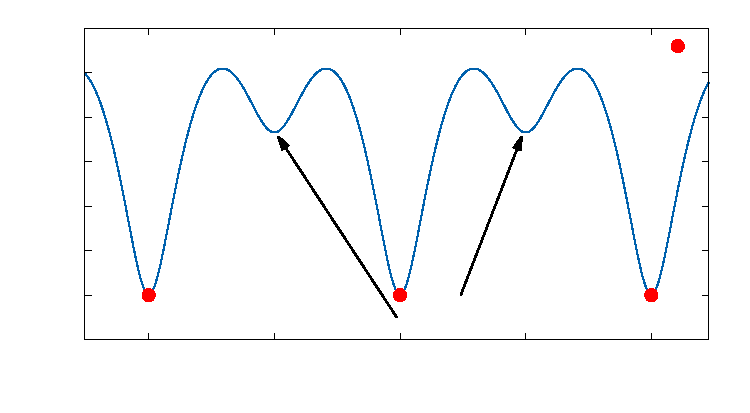
\includegraphics{gp/plotpga-eps-converted-to.pdf}}%
    \gplfronttext
  \end{picture}%
\endgroup
}
%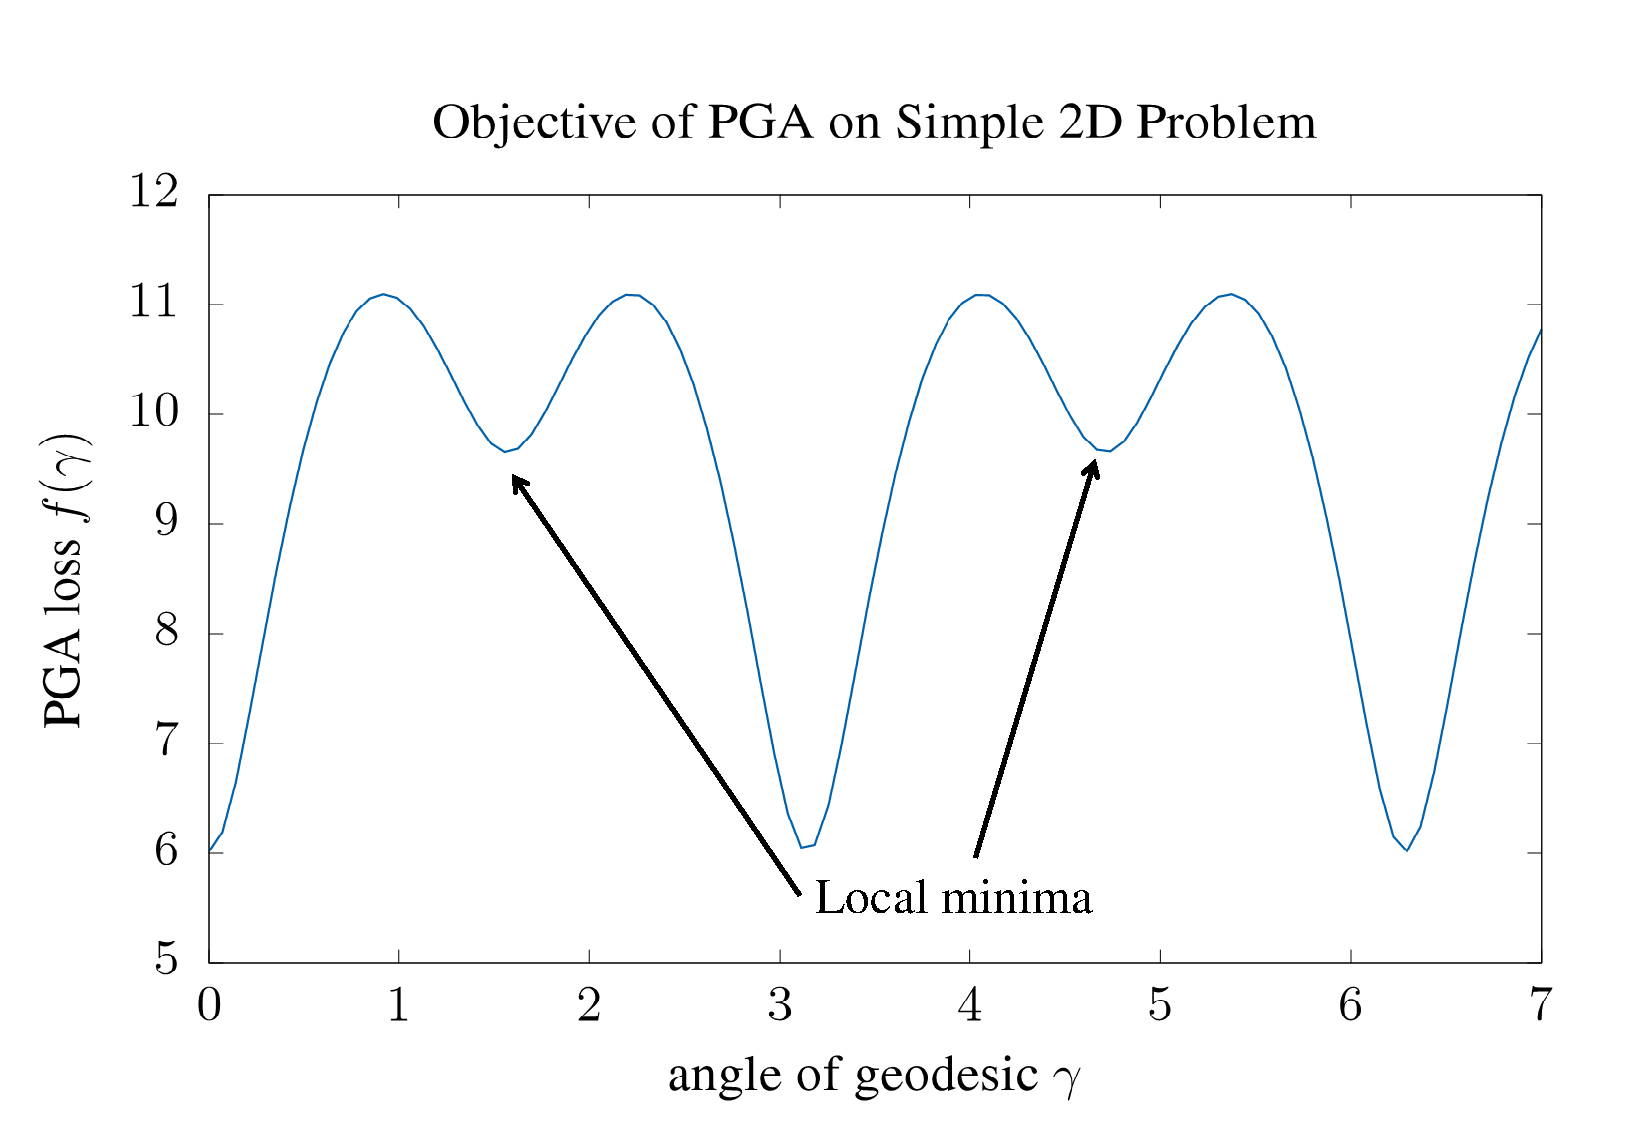
\includegraphics[width=0.3\textwidth]{gp/plotpga-labeled}
\caption{The PGA objective of an example task where the input dataset in the Poincar{\'e} disk is $x_1 = (0.8,0)$, $x_2 = (-0.8,0)$, $x_3 = (0,0.7)$ and $x_4 = (0,-0.7)$. Note the presence of non-optimal local minima, unlike PCA.}
\label{fig:pga}
\end{figure}

Nevertheless, there will always be a region $\Omega$ containing a
global optimum $\gamma^*$ that is convex and admits an efficient
projection, and where $f$ is convex when restricted to $\Omega$. Thus
it is possible to build a gradient descent-based algorithm to recover
lower-dimensional subspaces: for example, we built a simple optimizer
in PyTorch.  We also give a sufficient condition on the data for $f$ above
to be convex.
\begin{lemma}
For hyperbolic PGA if for all $i$,
\[
  \acosh^2\left( 1 + d_{E}(\gamma,w_i)^2 \right) < \min\left(1, \frac{1}{3} \| w_i \|^2 \right)
\]
then $f$ is locally convex at $\gamma$.
\label{lemma:pga}
\end{lemma}
As a result, if we initialize in and optimize over a region that
contains $\gamma^*$ and where the condition of Lemma~\ref{lemma:pga}
holds, then gradient descent will be guaranteed to converge to
$\gamma^*$. We can turn this result around and read it as a recovery
result: if the noise is bounded in this regime, then we are able to
provably recover the correct low-dimensional embedding.


% Another way of solving PGA is to approximate $f(\gamma)$ with a series of Euclidean PCA problems.
% Since the function $h(\beta) = \acosh^2(1 + \beta)$ is concave, for any $\gamma_0$
% \[
%   f(\gamma)
%   \le
%   \frac{1}{4} \sum_{i=1}^n
%   h'\left( d_{E}^2(\gamma_0,v_i)^2 \right)
%   d_{E}^2(\gamma,v_i)^2
%   +
%   R(\gamma_0, v_i)
% \]
% for some remainder $R$ that is independent of $\gamma_0$.
% This upper bound can be minimized over $\gamma$ as a weighted PCA problem, and by repeating this procedure we can converge to the optimum.

% not sure if we have space for the rest of the analysis here

%In this section, we consider how to reduce the dimensionality of embeddings. That is, we are given an embedding and wish to find a lower-rank version.
%%In Euclidean space, one can get the optimal lower rank embedding by simply discarding components. However, this may not be the case in hyperbolic space.
%%We describe a sufficient condition for dimensionality reduction to work and analyze the underlying issues. 
%
%%\begin{tcolorbox}
%%{\bf Takeaway}: Reoptimize lower dimensional embeddings.
%%\end{tcolorbox}
%
%%We work in $\mathbb{H}_2$ for simplicity, but the ideas in this section extend to higher dimensions. We are given an initial embedding 
%with points $x_1,\dots,x_n \in \mathbb{H}_2$. Our goal is to find a geodesic $\gamma : [0,1] \to \mathbb{H}_2$ that minimizes the
%variance to the points
%    \[ f(\gamma) = \sum_{i=1}^n \min_{t \in [0,1]} d_{H}(\gamma(t),x_i)^2 .\]
%    
%A major challenge that we face is that \emph{the loss function is not convex}. We observe that there
%  are multiple local minima {\color{red}PLOT}. Moreover, notice these losses are
%   attractive and stable, in contrast to analogous settings like PCA.
%
%\begin{tcolorbox}
%{\bf Takeaway}:   The underlying optimization may be nonconvex and this issue is not easily handled.
%\end{tcolorbox}
%
% {\color{red}NEEDS WRITTEN}.
%We begin by reducing the problem to one in Euclidean geometry. The key observation is that geodesics through the origin are just lines. 
%Therefore we use two steps to perform the reduction: (i) center the problem and then (ii) simplify the loss using the simpler geometry at the origin.
%The centering is done by computing the mean (known as the Frechet or Karcher
%mean)  efficiently using existing algorithms
%  
%In the Euclidean setting, we seek to find the line that minimizes the hyperbolic distances to
%  that line. The closest point to a line is half the distance of its reflection. Moreover,
%    any line is a geodesic in both Euclidean and hyperbolic geometry, hence:
%    \[ \min_{t} d_{H}(\gamma(t),x) = \frac{1}{2} \mathsf{acosh}\left(1 + \frac{d_{E}^2(l,x)}{ (1-\|x\|^2)^2 }\right) \]
%     Here, we have also used the fact that a point and its reflection have the
%     same norm. Now our expression is in terms of the Euclidean distance
%     to the line.
%
%Next, observe that we can normalize the points $v_i =
%       \frac{x_i}{1-\|x_i\|^2}$ to rewrite the above cost as $ \frac{1}{2} \mathrm{acosh}(1 + d^2_E(l,v_i) )$.
%        
%Intuitively, if there is such a line such that it's
%  variances to all points are small, then we should be able to recover
%  it. More precisely, we are looking for a set $\Omega \subseteq
%  \mathbb{S}^2$ that has three properties: (i) If there is a solution $u_*$ such that $f(u_*) = 0$, then
%      $\Omega$ contains $u_*$.(ii) The set $\Omega$ is a convex and admits an efficient projection. (iii) The loss $f$ is convex restricted to the set $\Omega$. Here,
%      \[ f(u) = \sum_{i=1}^{n} \min d_{H}( \ell(u),x_i)^2. \]
%
%We show that if there is a solution $u_*$ such that
%  \[ \sum_{i=1}^{n} r_i(u_*) \leq \min \{1, \frac{1}{3}\|v_i\|^2 \}. \]
%
%%Note that PCA does the wrong thing on the following example:
% % There are four points $y_{i} = \pm \alpha e_1$ (two of each) and two
% % of $x_i = \beta e_2$. Hence, the PCA loss for chosing $e_1$ is
% % $2\beta^2$ versus $4\alpha^2$ versus the $2\acosh(1+\beta^2)$ versus
% % $4\acosh(1+\alpha^2)^2$. Thus, we need to find values in which:
%  %\[ \beta^2 < 2 \alpha^2 \text{ and }  \acosh(1+\beta^2)^2 > 2\acosh(1+\alpha^2)^2 \]
%  %Take values like $\alpha = 5$ and $\beta = 10$.
%  
%%  We show that so long as there is a solution $u_*$ such that
%%  (\yell{see condition below}.)
%
%Thus we introduce the following straightforward algorithm.
%  \begin{itemize}
%\item Normalize the data as described in the note.
%  \item find a direction $u$:
%  \[ \min_{u \in \mathbb{S}^{n-1}} \max_{i} \|(I-uu^T)x_i\|^2 \]
%\item If the objective value is greater than $\frac{1}{3}$, fail.
%  \item If the objective value is smaller, then run projected gradient
%    descent with $P_{\Omega}$ as the projection on the original
%    function initialized with $u$.
%  \end{itemize}

%
%\subsection{Computing Derivatives}
%
%\[ r_i(u) = \| w - \|u\|^{-2}u (u \cdot w)\|^2 = \|w\|^2 - \|u\|^{-2} (u \cdot w)^2 \]
%\begin{align*}
%  h(x) = & \acosh(1+x)^2\\
%  h'(x) = & 2\acosh(1+x)(x^2 + 2x)^{-1/2}\\
%  h''(x) = & 2\left(\frac{1}{x^2 + 2x} - \acosh(1+x)(x^2 + 2x)^{-3/2}(x+1)\right)\\
%         = & 2\left(\frac{q^{1/2} - \acosh(1+x)(x+1)}{q^{3/2}}\right)\\
%  r_i(u) = & \|w_i\|^2 - (u\cdot w_i)^2 \|u\|^{-2}\\
%  r_i'(u) = & 2\|u\|^{-2} (u\cdot w_i) \left((u\cdot w_i) \|u\|^{-2} u - w_i \right) = 2\|u\|^{-2} (u\cdot w_i) (\|u\|^{-2}uu^T - I)w\\
%  r_i''(u) = & - 2w_i w_i^T \dots\\
%  f(u) = & \sum_{i=1}^{n} h(r_i(u))\\
%  f'(u) = & \sum_{i=1}^{n} h'(r_i(u))r'_i(u)\\
%  f''(u) = & \sum_{i=1}^{n} h''(r_i(u)) r'_i(u)r_i'(u)^T + h'(r_i(u))r_i''(u)\\
%  = & 2\sum_{i=1}^{n} \left(h''(r_i(u)) 2(u \cdot w_i)^2 - h'(r_i(u))\right) w_iw_i^T\\
%  = & 2\sum_{i=1}^{n} \left(h''(r_i(u)) 2(\|w_i\|^2-r_i(u)) - h'(r_i(u))\right) w_iw_i^T
%\end{align*}
%Let's do the angular version:
%\begin{align*}
%  \rho_i(\theta) = &  \|w_i\|^2(1 - \cos(\theta-\theta_i)^2) = \|w_i\|^2 \sin^2(\theta-\theta_i)\\
%  \rho_i'(\theta)= & 2 \|w_i\|^2 \sin(\theta-\theta_i) \cos(\theta-\theta_i) = \|w_i\|^2 \sin(2(\theta-\theta_i))\\
%  \rho_i''(\theta)= & 2 \|w_i\|^2 \cos(2(\theta-\theta_i))\\
%  g(\theta) = & \sum_{i=1}^{n} h(\rho_i(\theta))\\
%  g'(\theta) = & \sum_{i=1}^{n} h'(\rho_i(\theta)) \rho_i(\theta)\\
%  g''(\theta) = & \sum_{i=1}^{n} h''(\rho_i(\theta)) (\rho'_i(\theta))^2 + h'(\rho_i(\theta)) \rho''_i(\theta)\\
%  = &  \sum_{i=1}^{n} 4 \|w_i\|^4 \sin^2(2(\theta-\theta_i)) h''(\rho_i(\theta)) + 2 \|w_i\|^2 \cos(2(\theta-\theta_i)) h'(\rho_i(\theta))\\
%\end{align*}
%
%Observe that $\lim_{x \to 0} h'(x) =  2\frac{\acosh(1+x)}{\sqrt{x^2 + x}} = 2$. 
%\subsubsection{Estimates}
%
%{\bf Proposition}.  Using the notation above, 
%  \[ |\theta_i - \theta| \leq \frac{\pi}{7} \min \{ 1, \|w_i\|^{-1} \} \text{ then }
%  \frac{\partial^2}{\partial^2 \theta} h(\rho_i(\theta_i - \theta)) \geq 0
%  \] 
%
%\begin{proof}[Sketch]
%Let $\|w_i\| = t$ and, abusing notation, we write $\theta = \theta_i - \theta$ below. We show
%that when $t \leq 1$, then as long as $\theta \leq \pi/7$, then the
%term is positive definite.  We first consider when $\|w_\| = t \leq 1$
%then $h'(\rho_i(\theta)) \in [1.5,2]$ then, the second term is
%$[3t^2\cos(2\theta),4t^2\cos(2\theta)]$. We also observe that
%$h''(\rho_i(\theta)) \in [-\frac{2}{3}, -\frac{1}{3}]$. Hence, the
%lower bound for the whole term is:
%\[ \cos(2\theta) \geq \frac{8}{9} t^2 \sin^2(2\theta) \]
%Thus, this inequality holds (easily) if $\theta \in [-\pi/7,\pi/7]$.
%
%The lower bound on $h''$ still holds, hence we have:
%\[ \frac{4}{3} t^2 \sin^2(2\theta) \leq \cos(2\theta) h'(\rho(\theta)) \]
%
%For $t \geq 1$, if we insist $|\theta| \leq \pi/(7t)$ then $h'(\rho(\theta)) \geq 15/8$ and we have:
%\[ \frac{32}{45} t^2 \sin^2(2\theta) \leq \cos(2\theta) \]
%
%Note that $\sin(2\theta)^2 \leq \left(\pi/(7t)\right)^2$. It is
%straightforward to verify that the left hand side is less than $0.6$,
%while $\cos(2\pi/7) > 0.6$--and the rhs is an increasing function of $t$.
%
%\end{proof}
%
%Note that for large $t$, $\rho(t,\theta) = O(1)$ and that a constant fraction 



\section{Experiments}
\label{sec:experiments}
\vspace{-0.2cm}
\section{Experiments Details}
\label{sec:exp}

\vspace{-0.2cm}
\subsection{Roadmap Insights on FFHQ-256\texorpdfstring{~\cite{sg1}}{}}
\label{sub:arc-experiments}
\vspace{-0.1cm}
As per Table~\ref{tab:roadmap}, Config A (vanilla StyleGAN2) achieves an FID of 7.52 using the official implementation on FFHQ-256. Config B with all tricks removed achieves an FID of 12.46---performance drops as expected. 
Config C, with a well-behaved loss, achieves an FID of 11.65. But, now training is sufficiently stable to improve the architecture.

Config D, which improves $G$ and $D$ based on the classic ResNet and ConvNeXt findings, achieves an FID of 9.95. The output skips of the StyleGAN2 generator are no longer useful given our new architecture; including them produces a worse FID of 10.17. Karras~\etal find that the benefit of output skips is mostly related to gradient magnitude dynamics~\cite{sg3}, and this has been addressed by our ResNet architecture. For StyleGAN2, Karras~\etal conclude that a ResNet architecture is harmful to $G$~\cite{sg2}, but this is not true in our case as their ResNet implementation is considerably different from ours: 1) Karras~\etal use one 3-3 residual block for each resolution stage, while we have a separate transition layer and two 1-3-1 residual blocks; 2) i.3) and i.4) are violated as they do not have a linear residual block~\cite{mobnet} and the transition layer is placed on the skip branch of the residual block rather than the stem; 3) the essential principle of ResNet~\cite{resnet}---identity mapping~\cite{resnet2}---is violated as Karras~\etal divide the output of the residual block by $\sqrt{2}$ to avoid variance explosion due to the absence of a proper initialization scheme.

For Config E, we conduct two experiments that ablate i.\ref{item:i1} (increased width with depthwise conv.) and i.\ref{item:i2} (an inverted bottleneck). We add GroupedConv and reduce the bottleneck compression ratio to two given the same model size. Each bottleneck is now 1.5$\times$ the width of Config A, and the FID drops to 7.51, surpassing the performance of StyleGAN2. By inverting the stem and the bottleneck dimensions to enhance the capacity of GroupedConv, our final model achieves an FID of 7.05, exceeding StyleGAN2.


\begin{wraptable}[12]{r}{6.5cm}
\vspace{-1.25cm}
\centering
\caption{StackedMNIST 1000-mode coverage.}
% Our model outperforms other GANs in terms of $D_\text{KL}$, indicating that we are better able to recover the distribution.}
\vspace{-0.4cm}
\resizebox{0.8\linewidth}{!}{
\begin{tblr}{
  cell{2}{2} = {c},
  cell{2}{3} = {c},
  cell{3}{2} = {c},
  cell{3}{3} = {c},
  cell{4}{2} = {c},
  cell{4}{3} = {c},
  cell{5}{2} = {c},
  cell{5}{3} = {c},
  cell{6}{2} = {c},
  cell{6}{3} = {c},
  cell{7}{2} = {c},
  cell{7}{3} = {c},
  cell{8}{2} = {c},
  cell{8}{3} = {c},
  cell{9}{2} = {c},
  cell{9}{3} = {c},
  cell{10}{2} = {c},
  cell{10}{3} = {c},
  cell{11}{2} = {c},
  cell{11}{3} = {c},
  cell{12}{2} = {c},
  cell{12}{3} = {c},
  hline{2,12} = {1-3}{},
}
Model     & \# modes$\uparrow$ & $D_\text{KL}$$\downarrow$            &  \\
DCGAN~\cite{dcgan}     & 99            & 3.40\phantom{0}&  \\
VEEGAN~\cite{srivastava2017veegan}    & 150           & 2.95\phantom{0}&  \\
WGAN-GP~\cite{wgan-gp}& 959           & 0.73\phantom{0}&  \\
PacGAN~\cite{pacgan}    & 992           & 0.28\phantom{0}&  \\
StyleGAN2~\cite{sg2} & 940           & 0.42\phantom{0}&  \\
PresGAN~\cite{presgan}   & \textbf{1000} & 0.12\phantom{0}&  \\
Adv. DSM~\cite{advsm}  & \textbf{1000} & 1.49\phantom{0}&  \\
VAEBM~\cite{vaebm}     & \textbf{1000} & 0.087          &  \\
DDGAN~\cite{ddgan}     & \textbf{1000} & 0.071          &  \\
MEG~\cite{meg}       & \textbf{1000} & 0.031          &  \\
Ours---Config E     & \textbf{1000} & \textbf{0.029} &  
\end{tblr}
}
\label{tab:stackedmnist}
\end{wraptable}%

\subsection{Mode Recovery --- StackedMNIST\texorpdfstring{~\cite{metz2016unrolled}}{}} 
\vspace{-0.1cm}
We repeat the earlier experiment in 1000-mode convergence on StackedMNIST (unconditional generation), but this time with our updated architecture and with comparisons to SOTA GANs and likelihood-based methods (Tab.~\ref{tab:stackedmnist}, Fig.~\ref{fig:stacked-mnist}). 
One advantage brought up of likelihood-based models such as diffusion over GANs is that they achieve mode coverage~\cite{adm}. We find that most GANs struggle to find all modes. But, PresGAN~\cite{presgan}, DDGAN~\cite{ddgan}, and our approach are successful. Further, our method outperforms all other tested GAN models in term of KL divergence.

\subsection{FID --- FFHQ-256\texorpdfstring{~\cite{sg1}}{} (Optimized)}
\vspace{-0.1cm}
We train Config E model until convergence and with optimized hyperparameters and training schedule on FFHQ at 256$\times$256 (unconditional generation) (Tab.~\ref{tab:ffhq256}, Figs.~\ref{fig:ffhq-256-teaser} and~\ref{fig:ffhq-256}). 
Please see our supplemental material for training details.
%The hyperparameters and schedule are listed in the supplemental material. 
Our model outperforms existing StyleGAN methods, plus four more recent diffusion-based methods. On this common dataset experimental setting, many methods (not listed here) use the bCR~\cite{zhao2021improved} trick---this has only been shown to improve performance on FFHQ-256 (not even at different resolutions of FFHQ)~\cite{zhao2021improved, zhang2022styleswin}. We do not use this trick. 
% no such tricks in our method.
% JT Try to minimize embellishment...
% This is particularly impressive given the fact that the dataset FFHQ was designed for StyleGAN~\cite{sg1} and the StyleGAN series of models were optimized with this specific dataset in mind.
% to achieve this performance.

\subsection{FID --- FFHQ-64\texorpdfstring{~\cite{edm}}{}}
\vspace{-0.1cm}
To compare with EDM~\cite{edm} directly, we evaluate our model on FFHQ at 64$\times$64 resolution. For this, we remove the two highest resolution stages of our 256$\times$256 model, resulting in a generator that is less than half the number of parameters as EDM. Despite this, our model outperforms EDM on this dataset and needs one function evaluation only (Tab.~\ref{tab:ffhq64}).

\begin{figure}
\begin{floatrow}
    %\hspace{-0.75cm}%
    \capbtabbox{%
        \centering
        \resizebox{\linewidth}{!}{
        \begin{tblr}{
          column{2,3} = {r},
          cell{1}{2} = {c},
          cell{1}{3} = {c},
          hline{2,5,9,10} = {-}{},
        }
        Model       & NFE$\downarrow$ & FID$\downarrow$  \\
        StyleGAN2~\cite{sg2}   & 1               & 3.78 \\
        StyleGAN3-T~\cite{sg3} & 1               & 4.81 \\
        StyleGAN3-R~\cite{sg3} & 1               & 3.92 \\
        LDM~\cite{rombach2022high} & 200               & 4.98\\
        ADM (DDIM)~\cite{adm,compdiff} & 500               & 8.41\\
        ADM (DPM-Solver)~\cite{adm,compdiff} & 500               & 8.40\\
        Diffusion Autoencoder~\cite{diffae,compdiff} & 500               & 5.81\\
        Ours---Config E  & 1               & 2.75 \\
        \emph{With ImageNet feature leakage~\cite{kynkaanniemi2022role}:} & & \\
        PolyINR*~\cite{singh2023polynomial} & 1               & 2.72 \\
        StyleGAN-XL*~\cite{sgxl} & 1               & 2.19 \\
        StyleSAN-XL*~\cite{takida2024san} & 1               & 1.68 \\
        \end{tblr}
        }
    }{%
        \caption{
        \label{tab:ffhq256}FFHQ-256. * denotes models that leak ImageNet features.}
    }
    %
    \capbtabbox{%
        \centering
        \resizebox{0.85\linewidth}{!}{
        \begin{tblr}{
          column{2} = {r},
          column{3} = {r},
          hline{2,5,8} = {-}{},
        }
        Model         & NFE$\downarrow$ & FID$\downarrow$ \\
        StyleGAN2~\cite{sg2,anycostgan}     & 1               & 3.32            \\
        MSG-GAN~\cite{karnewar2020msg,anycostgan}       & 1               & 2.7             \\
        Anycost GAN~\cite{anycostgan}   & 1               & 2.52            \\
        VE~\cite{sde,edm}            & 79              & 25.95           \\
        VP~\cite{sde,edm}            & 79              & 3.39            \\
        EDM~\cite{edm}           & 79              & 2.39            \\
        Ours—Config E & 1               & 1.95 \\
        \end{tblr}
        }
    }{%
        \caption{\label{tab:ffhq64}FFHQ-64.}
    }
\end{floatrow}
\vspace{-0.25cm}
\end{figure}


% \begin{figure}
% \begin{floatrow}
%     \capbtabbox{%
%         \centering
%         \resizebox{0.8\linewidth}{!}{
%         \begin{tblr}{
%           column{2,3} = {r},
%           cell{1}{2} = {c},
%           cell{1}{3} = {c},
%           hline{2,9,13} = {-}{},
%         }
%         Model               & NFE$\downarrow$ & FID$\downarrow$ \\
%         BigGAN~\cite{biggan}              & 1               & 14.73 \\
%         TransGAN~\cite{trans}            & 1               & 9.26 \\
%         ViTGAN~\cite{vitgan}              & 1               & 6.66 \\
%         DDGAN~\cite{ddgan}               & 4               & 3.75 \\
%         Diffusion StyleGAN2~\cite{diffusiongan} & 1               & 3.19 \\
%         StyleGAN2 + ADA~\cite{sg2ada}     & 1               & 2.42 \\
%         StyleGAN3-R + ADA~\cite{sg3,studio}   & 1               & 10.83 \\
%         DDPM~\cite{ddpm}               & 1000            & 3.21 \\
%         DDIM~\cite{ddim}                & 50             & 4.67 \\
%         VE~\cite{sde,edm}                  & 35              & 3.11 \\
%         VP~\cite{sde,edm}                  & 35              & 2.48 \\
%         Ours---Config E     & 1               & 1.96 \\
%         \hline
%         \emph{With ImageNet feature leakage~\cite{kynkaanniemi2022role}:} & & \\
%         StyleGAN-XL*~\cite{sgxl}       & 1               & 1.85 \\
%         \end{tblr}
%         }
%     }{%
%         \caption{\label{tab:cifar10}CIFAR-10.}
%     }
%         % \begin{tblr}{
%         %   column{2,3} = {r},
%         %   cell{1}{2}{3} = {},
%         %   hline{2,9,13} = {-}{},
%         % }
%         % Model               & FID$\downarrow$ & Params          \\
%         % BigGAN~\cite{biggan}              & 14.73  & --       \\
%         % TransGAN~\cite{trans}            & 9.26 & --         \\
%         % ViTGAN~\cite{vitgan}              & 6.66 & --         \\
%         % DDGAN~\cite{ddgan}               & 3.75 & --         \\
%         % Diffusion StyleGAN2 & 3.19 & 40.1M           \\
%         % StyleGAN2 + ADA     & 2.42 & 40.1M          \\
%         % StyleGAN3-R + ADA   & 10.83 & 40.1M        \\
%         % DDPM               & 3.21 & 35.2M         \\
%         % DDIM                & 4.67 & --         \\
%         % VE~\cite{edm}                  & 3.11 & 61.8M        \\
%         % VP~\cite{edm}                  & 2.48 & 61.8M         \\
%         % Ours---Config E     & \textbf{1.99}  & 43.0M \\
%         % StyleGAN-XL*~\cite{sgxl}       & 	1.85 & 140.0M \\
%         % \end{tblr}
        
%     %     }
%     % }{%
%     %     \caption{\label{tab:cifar10}CIFAR-10.}
%     % }%
%     %\hspace{-0.75cm}%
%     %\hspace{-0.5cm}%
% \end{floatrow}
% \end{figure}

\subsection{FID --- CIFAR-10~\cite{krizhevsky2009learning}} \vspace{-0.1cm}

\begin{wraptable}[14]{r}{6.5cm}
\vspace{-0.75cm}
\centering
\caption{\label{tab:cifar10}CIFAR-10 performance.}
\vspace{-0.4cm}
\resizebox{0.9\linewidth}{!}{
    \begin{tblr}{
          column{2,3} = {r},
          cell{1}{2} = {c},
          cell{1}{3} = {c},
          hline{2,9,13} = {-}{},
        }
        Model               & NFE$\downarrow$ & FID$\downarrow$ \\
        BigGAN~\cite{biggan}              & 1               & 14.73 \\
        TransGAN~\cite{trans}            & 1               & 9.26 \\
        ViTGAN~\cite{vitgan}              & 1               & 6.66 \\
        DDGAN~\cite{ddgan}               & 4               & 3.75 \\
        Diffusion StyleGAN2~\cite{diffusiongan} & 1               & 3.19 \\
        StyleGAN2 + ADA~\cite{sg2ada}     & 1               & 2.42 \\
        StyleGAN3-R + ADA~\cite{sg3,studio}   & 1               & 10.83 \\
        DDPM~\cite{ddpm}               & 1000            & 3.21 \\
        DDIM~\cite{ddim}                & 50             & 4.67 \\
        VE~\cite{sde,edm}                  & 35              & 3.11 \\
        VP~\cite{sde,edm}                  & 35              & 2.48 \\
        Ours---Config E     & 1               & 1.96 \\
        \hline
        \emph{With ImageNet feature leakage~\cite{kynkaanniemi2022role}:} & & \\
        StyleGAN-XL*~\cite{sgxl}       & 1               & 1.85 \\
        \end{tblr}
}
\end{wraptable}

We train Config E model until convergence and with optimized hyperparameters and training schedule on CIFAR-10 (conditional generation) (Tab.~\ref{tab:cifar10}, Fig.~\ref{fig:cifar10}). Our method outperforms many other GANs by FID even though the model has relatively small capacity. For instance, StyleGAN-XL~\cite{sgxl} has 18\ M parameters in the generator and 125\ M parameters in the discriminator, while our model has a 40\ M parameters between the generator and discriminator combined (Fig.~\ref{fig:fid-50k-vs-params-cifar-10}). Compared to diffusion models like LDM or ADM, GAN inference is significantly cheaper as it requires only one network function evaluation compared to the tens or hundreds of network function evaluations for diffusion models without distillation. 

\begin{wrapfigure}[12]{r}{6.5cm}
    \vspace{-0.4cm}
    \centering
    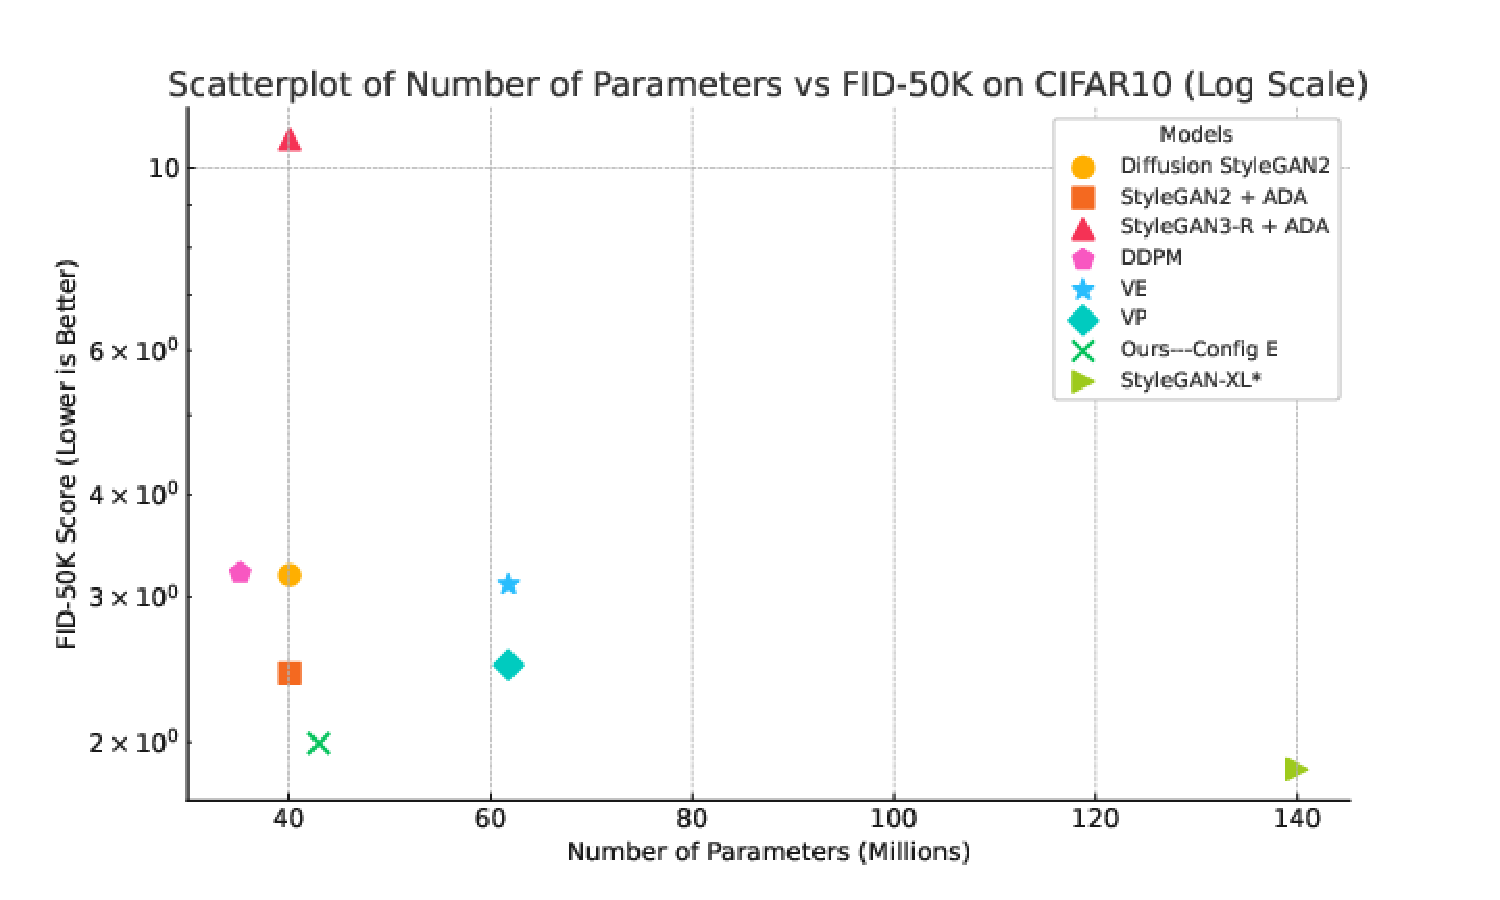
\includegraphics[width=\linewidth,clip,trim={0 0 0 2cm}]{figures/Scatterplot-FID-Parameters-CIFAR10.pdf}
    \caption{Millions of parameters vs.~FID-50K (log scale) on CIFAR-10. Lower is better.}
    \label{fig:fid-50k-vs-params-cifar-10}
\end{wrapfigure}

Many state-of-the-art GANs are derived from Projected GAN~\cite{sauer2021projected}, including StyleGAN-XL~\cite{sgxl} and the concurrent work of StyleSAN-XL~\cite{takida2024san}. These methods use a pre-trained ImageNet classifier in the discriminator. Prior work has shown that a pre-trained ImageNet discriminator can leak ImageNet features into the model~\cite{kynkaanniemi2022role}, causing the model to perform better when evaluating on FID since it relies on a pre-trained ImageNet classifier for the loss. But, this does not improve results in perceptual studies~\cite{kynkaanniemi2022role}. Our model produces its low FID without any ImageNet pre-training.

%\jt{Missing citations here for such methods.}


%\aaron{add NFEs}
%\jt{Which models in our evaluation use this? Any?}

%\jt{What is the second caveat?}

\subsection{FID --- ImageNet-32~\cite{chrabaszcz2017downsampled}}
\label{sec:imagenet32-fid-explain}
We train Config E model until convergence and with optimized hyperparameters and training schedule on ImageNet-32 (conditional generation). We compare against recent GAN models and recent diffusion models in Table~\ref{tab:imagenet32}.
We adjust the number of parameters in the generator of our model to match StyleGAN-XL~\cite{sgxl}'s generator (84M parameters). Specifically, we make the model significantly wider to match. Our method achieves comparable FID despite using a 60\% smaller discriminator (Tab.~\ref{tab:imagenet32}) and despite not using a pre-trained ImageNet classifier.
%, which has been shown to improve FID performance, but not improve results in perceptual studies~\cite{kynkaanniemi2022role}.

\vspace{-0.1cm}
\subsection{FID --- ImageNet-64~\cite{chrabaszcz2017downsampled}}
We evaluate our model on ImageNet-64 to test its scalability. We stack another resolution stage on our ImageNet-32 model, resulting in a generator of 104\ M parameters. This model is nearly 3$\times$ smaller than diffusion-like models~\cite{adm,edm,cm,icm} that rely on the ADM backbone, which contains about 300\ M parameters. Despite the smaller model size and that our model generates samples in one step, it outperforms larger diffusion models with many NFEs on FID (Tab.~\ref{tab:imagenet64}).

\vspace{-0.1cm}
\subsection{Recall}
We evaluate the recall~\cite{precrecall} of our model on each dataset to quantify sample diversity. In general, our model achieves a recall that is similar to or marginally worse than the diffusion model counterpart, yet superior to existing GAN models. For CIFAR-10, the recall of our model peaked at 0.57; as a point of comparison, StyleGAN-XL~\cite{sgxl} has a worse recall of 0.47 despite its lower FID. For FFHQ, we obtain a recall of 0.53 at 64$\times$64 and 0.49 at 256$\times$256, whereas StyleGAN2~\cite{sg2} achieved a recall of 0.43 on FFHQ-256. Our ImageNet-32 model achieved a recall of 0.63; comparable to ADM~\cite{adm}. Our ImageNet-64 model achieved recall 0.59. While this is slightly worse than $\approx$0.63 that many diffusion models achieve, it is better than BigGAN-deep~\cite{biggan} which achieved a recall of 0.48.

\begin{figure}
    \begin{floatrow}
        \capbtabbox{%
        \centering
        \resizebox{0.9\linewidth}{!}{
        \begin{tblr}{
          column{2} = {r},
          column{3} = {r},
          cell{8}{1} = {c=3}{},
          hline{2,7-8} = {-}{},
        }
    Model                                                       & NFE$\downarrow$  & FID$\downarrow$                        \\ 
    DDPM++~\cite{kim2021soft}                  & 1000 & 8.42                                   \\
    VDM~\cite{kingma2021variational}           & 1000 & 7.41                                   \\
    MSGAN~\cite{karnewar2020msg,ning2023input} & 1    & 12.3                                   \\
    ADM~\cite{adm}                             & 1000 & 3.60                                   \\
    DDPM-IP~\cite{ning2023input}               & 1000 & 2.87                                   \\
    Ours—Config E               & 1    & 1.27   \\
    \textit{With ImageNet feature leakage~\cite{kynkaanniemi2022role}:}    \\
    StyleGAN-XL*~\cite{sgxl}                   & 1    & 1.10                                  
    \end{tblr}
        }
    }{%
        \caption{\label{tab:imagenet32}ImageNet-32.}
        % \jt{some are conditional still}}
    }
    %
    \capbtabbox{
        \centering
        \resizebox{0.9\linewidth}{!}{
        \begin{tblr}{
          column{2} = {r},
          column{3} = {r},
          cell{1}{2} = {c},
          cell{1}{3} = {c},
          cell{12}{1} = {c=3}{},
          hline{2-3,11-12} = {-}{},
        }
        Model         & NFE$\downarrow$ & FID$\downarrow$ \\
        BigGAN-deep~\cite{biggan}\phantom{xx}   & 1               & 4.06            \\
        DDPM~\cite{ddpm}          & 250             & 11.0            \\
        DDIM~\cite{ddim}          & 50              & 13.7            \\
        ADM~\cite{adm}           & $^\S$250             & 2.91            \\
        EDM~\cite{edm}           & 79              & 2.23            \\
        CT~\cite{cm}            & 2               & 11.1            \\
        CD~\cite{cm}            & 3               & 4.32            \\
        iCT-deep~\cite{icm}      & 2               & 2.77            \\
        DMD~\cite{dmd}           & 1               & 2.62            \\
        Ours—Config E & 1               & 2.09            \\
        \emph{With ImageNet feature leakage~\cite{kynkaanniemi2022role}:}          &                 &                 \\
        StyleGAN-XL*~\cite{sgxl}   & 1               & 1.52            
        \end{tblr}
        }
    }
    {
        \caption{\label{tab:imagenet64}ImageNet-64.\hspace{-0.1cm} {\small \S:\hspace{-0.05cm}deterministic sampling.}}
    }
    \end{floatrow}
    \vspace{-0.25cm}
\end{figure}


% \begin{table}[ht]
%     \centering
%     \begin{tabular}{lcccccccc}
%         \toprule
%         \textbf{Model} & \textbf{\# Param.} & \textbf{IS $\uparrow$} & \textbf{FID $\downarrow$} & \textbf{Precision $\uparrow$} & \textbf{Recall $\uparrow$} & \textbf{Density $\uparrow$} & \textbf{Coverage $\uparrow$} & \textbf{Inf. (s)} \\
%         \midrule
%         ReACGAN + DiffAug (Ours) [10] & 9.4M & 10.15 & 2.64 & 0.75 & 0.65 & 0.98 & 0.90 & 0.009 \\
%         StyleGAN2-ADA [85] & 20.2M & 10.31 & 2.41 & 0.74 & 0.68 & 1.02 & 0.92 & 0.008 \\
%         StyleGAN2-ADA (Ours) [85] & 20.2M & \textbf{10.53} & 2.31 & 0.75 & 0.69 & 1.04 & 0.93 & 0.008 \\
%         StyleGAN2 + DiffAug + D2D-CE (Ours) [10] & 20.2M & 10.46 & 2.30 & 0.76 & 0.68 & 1.03 & 0.93 & 0.007 \\
%         DDPM [43] & 35.2M & 9.73 & 3.23 & 0.78 & 0.67 & 1.10 & 0.93 & 15.422 \\
%         DDPM++ [44] & 106.6M & 9.90 & 2.49 & 0.78 & 0.69 & 1.12 & 0.94 & 46.697 \\
%         NCSN++ [44] & 107.6M & 10.08 & 2.27 & 0.77 & 0.70 & 1.07 & 0.94 & 99.304 \\
%         LSGM [45] & - & 10.04 & 2.80 & 0.80 & 0.70 & 1.15 & 0.95 & - \\
%         LSGM-ODE [45] & - & 10.07 & \textbf{2.09} & 0.77 & 0.71 & 1.03 & 0.94 & - \\
%         CLD-SGM [47] & - & 9.88 & 2.38 & 0.78 & 0.69 & 1.12 & 0.94 & - \\
%         StyleGAN-XL~ & 18.0M & \textbf{11.03} & \textbf{1.88} & 0.77 & 0.59 & 1.08 & 0.94 & 0.010 \\
%         % BaselineGAN & %10.284011840820312
%         % 10.28
%         % & %1.9925376117527978 
%         % 1.99 & % 0.6899600028991699 
%         % 0.69 &&
%         \bottomrule
%     \end{tabular}
%     \caption{Comparison of various models on CIFAR10 dataset. TODO fix citation}
% \label{tab:cifar10_comparison}
%\end{table}

% \jt{Is the below meant to be a conclusion? Some of these statements are unfounded in the evidence we present so far.}
% \begin{enumerate}

%     \item We demonstrate the ability of our method to recover all modes of training data on Stacked Mnist~\ref{tab:stackedmnist}.
%     \item We beat all methods that do not use bCR (shown to overfit for FFHQ-256~\cite{}) and methods that do not leak imagenet features from a pretrained discriminator~\cite{kynkaanniemi2022role}. If we exclude these two categories of models, we are SOTA across all open source GANs. We also SOTA on a per parameter count basis on multiple GANs.
%     \item We demonstrate SOTA performance on CIFAR-10 image generation at our current parameter count, outperforming all previous GANs except for StyleGAN-XL derived ones with X\% percent of the parameters of these methods. We also do not leak features from ImageNet or use a pretrained discriminator.~\ref{tab:cifar10}. 
%     \item We achieve near SOTA on FFHQ 256 and achieve SOTA for a GAN method without bCR or feature leakage.
%     \item We achieve near state of the art results on Imagenet and achieve Pareto frontier results for total GAN model parameter size.
% \end{enumerate}
% \begin{table}[h]
\centering
\caption{FID on ImageNet-32}
\begin{tabular}{ l c c }
\toprule
Model & \textbf{Year} & FID$\downarrow$ \\
\midrule
% %Real NVP (Dinh et al.) & 2016 & 4.28 \\
% %Glow (Kingma and Dhariwal) & 2018 & 4.09 \\
% %MintNet & 2019 & 4.06 \\
% % Residual Flow & 2019 & 4.01 \\
% % BIVA Maaloe et al. & 2019 & 3.96 \\
% % ANF Huang et al. & 2020 & 3.92 \\
% % NVAE w/ flow & 2020 & 3.92 \\
% % PixelRNN & 2016 & 3.86 \\
% % Flow++ & 2019 & 3.86 \\
% % SPN Menick and Kalchbrenner & 2018 & 3.85 \\
% % Gated PixelCNN & 2016 & 3.83 \\
% % Very Deep VAE & 2020 & 3.8 \\
% % MRCNF & 2021 & 3.77 \\
% % $\delta$-VAE & 2019 & 3.77 \\
% Image Transformer~\cite{parmar2018image} & 2018 & 3.77 \\
% ScoreFlow & 2021 & 3.76 \\
% Reflected Diffusion & 2023 & 3.74 \\
% %Hourglass & 2021 & 3.74 \\
% DenseFlow-74-10 & 2021 & 3.63 \\
% i-DODE & 2023 & 3.43 \\
% MSGAN~\cite{karnewar2020msg} & 2019 & 12.3 \\
% DDPM-IP & 2023 & 2.66 \\
MSGAN~\cite{karnewar2020msg} & 2019 & 12.3 \\
VDM~\cite{kingma2021variational} & 2021 & 7.41 \\
DDPM++~\cite{kim2021soft} & 2021 & 8.42 \\
DDPM-IP~\cite{ning2023input} & 2023 & 2.87 \\
\textbf{Ours} & 2024 & 1.28 \\
StyleGAN-XL~\cite{sauer2022stylegan} & 2022 & \textbf{1.10} \\
\bottomrule
\end{tabular}
\end{table}

% \begin{table}[tO]
%     \centering
%     \begin{tabular}{c|c|c|c}
%          & FID\_50k & Precision & Recall \\
%         StyleGAN &  \\
%         StyleGAN-XL? &
%         Lots of other baselines
%     \end{tabular}
%     \caption{Caption}
%     \label{tab:my_label}
% \end{table}
% \label{sec:exp}
% % cifar10, ffhq, imagenet

% \begin{table}
%     \centering
%     %\caption{Results for CIFAR-10 generation. \aaron{add NFEs}}
%     %\vspace{-2mm}
%     \begin{tblr}{
%       column{2} = {r},
%       cell{1}{2} = {c},
%       hline{2,9,13} = {-}{},
%     }
%     Model               & FID$\downarrow$           \\
%     BigGAN~\cite{biggan}              & 14.73         \\
%     TransGAN~\cite{trans}            & 9.26          \\
%     ViTGAN~\cite{vitgan}              & 6.66          \\
%     DDGAN~\cite{ddgan}               & 3.75          \\
%     Diffusion StyleGAN2 & 3.19          \\
%     StyleGAN2 + ADA     & 2.42          \\
%     StyleGAN3-R + ADA   & 10.83         \\
%     DDPM                & 3.21          \\
%     DDIM                & 4.67          \\
%     VE                  & 3.11          \\
%     VP                  & 2.48          \\
%     Ours---Config E     & \textbf{1.99} 
%     \end{tblr}
%     %\label{tab:cifar10}
%     \caption{Results for CIFAR-10 generation. \aaron{add NFEs}}
%     \label{tab:cifar10}
% \end{table}



%%%%%%%%%%%%%%%%%%%%%%%%%%%%%%%%%%%%%%%%%%%%%%%%%%%%%%%%%%%%%
% Qualitative figures
%%%%%%%%%%%%%%%%%%%%%%%%%%%%%%%%%%%%%%%%%%%%%%%%%%%%%%%%%%%%%

% Variable to control the size of each image
% \begin{figure}
%     \centering
%     \includegraphics{example-image-a}
%     \caption{stacked mnist (qualitative figure) (from powerpoint)}
%     \label{fig:stacked-mnist}
% \end{figure}
% cifar10, ffhq, imagenet

% \noindent\begin{minipage}{.33\textwidth}
% \centering
% \captionof{table}{1000-mode coverage on StackedMNIST.}
% \vspace{-2mm}
% \begin{tblr}{
%   cell{2}{2} = {c},
%   cell{2}{3} = {c},
%   cell{3}{2} = {c},
%   cell{3}{3} = {c},
%   cell{4}{2} = {c},
%   cell{4}{3} = {c},
%   cell{5}{2} = {c},
%   cell{5}{3} = {c},
%   cell{6}{2} = {c},
%   cell{6}{3} = {c},
%   cell{7}{2} = {c},
%   cell{7}{3} = {c},
%   cell{8}{2} = {c},
%   cell{8}{3} = {c},
%   cell{9}{2} = {c},
%   cell{9}{3} = {c},
%   cell{10}{2} = {c},
%   cell{10}{3} = {c},
%   cell{11}{2} = {c},
%   cell{11}{3} = {c},
%   hline{2,11} = {1-3}{},
% }
% Model     & Modes$\uparrow$ & KLD$\downarrow$            &  \\
% DCGAN     & 99            & 3.40\phantom{0}&  \\f
% VEEGAN    & 150           & 2.95\phantom{0}&  \\
% WGAN-GP   & 959           & 0.73\phantom{0}&  \\
% PacGAN    & 992           & 0.28\phantom{0}&  \\
% StyleGAN2 & 940           & 0.42\phantom{0}&  \\
% PresGAN   & \textbf{1000} & 0.12\phantom{0}&  \\
% Adv. DSM  & \textbf{1000} & 1.49\phantom{0}&  \\
% VAEBM     & \textbf{1000} & 0.087          &  \\
% DDGAN     & \textbf{1000} & 0.071          &  \\
% Ours      & \textbf{1000} & \textbf{???} &  
% \end{tblr}
% \label{tab:stackedmnist}
% \end{minipage}%
% \begin{minipage}{.33\textwidth}
% \centering
% \captionof{table}{Results for CIFAR-10 generation.}
% \vspace{-2mm}
% \begin{tblr}{
%   column{2} = {r},
%   cell{1}{2} = {c},
%   hline{2,9,13} = {-}{},
% }
% Model               & FID$\downarrow$           \\
% BigGAN              & 14.73         \\
% TransGAN            & 9.26          \\
% ViTGAN              & 6.66          \\
% DDGAN               & 3.75          \\
% Diffusion StyleGAN2 & 3.19          \\
% StyleGAN2 + ADA     & 2.42          \\
% StyleGAN3-R + ADA   & 10.83         \\
% DDPM                & 3.21          \\
% DDIM                & 4.67          \\
% VE                  & 3.11          \\
% VP                  & 2.48          \\
% Ours                & \textbf{1.99} 
% \end{tblr}
% \label{tab:cifar10}
% \end{minipage}%
% \begin{minipage}{.33\textwidth}
% \centering
% \captionof{table}{Results on FFHQ ($256\times256$).}
% \vspace{-2mm}
% \begin{tblr}{
%   column{2} = {r},
%   cell{1}{2} = {c},
%   hline{2,5} = {-}{},
%   hline{2,9} = {-}{},
% }
% Model       & FID$\downarrow$  \\
% StyleGAN2   & 3.78 \\
% StyleGAN3-T & 4.81 \\
% StyleGAN3-R & 3.92 \\
% LDM & 4.98\\
% ADM (DDIM) & 8.41\\
% ADM (DPM-Solver) & 8.40\\
% Diffusion Autoencoder & 5.81\\
% Ours        & \textbf{2.95} 
% \end{tblr}
% \label{tab:ffhq256}
% \end{minipage}


% \input{tables/cifar10}
% \input{tables/ffhq256}
% \input{tables/MNIST}
\begin{figure}[h!]
    \newlength{\imgsize}
    \setlength{\imgsize}{0.10\linewidth} % Adjust this value to change the size of the images
    
    % New command to include images from a specific directory
    \newcommand{\qualitativeimg}[1]{%
        \includegraphics[width=\imgsize]{figures/qualitative/ffhq-256-000139623/image-#1.jpg}%
    }
    
    \setlength{\tabcolsep}{0pt} % Remove spacing between columns
    \renewcommand{\arraystretch}{0} % Remove spacing between rows
    
    \centering
    \begin{tabular}{cccccccc} % Eight columns
        \qualitativeimg{64} & \qualitativeimg{65} & \qualitativeimg{66} & \qualitativeimg{67} & \qualitativeimg{128} & \qualitativeimg{69} & \qualitativeimg{70} & \qualitativeimg{71} \\
        \qualitativeimg{72} & \qualitativeimg{73} & \qualitativeimg{74} & \qualitativeimg{75} & \qualitativeimg{76} & \qualitativeimg{77} & \qualitativeimg{78} & \qualitativeimg{79} \\
        \qualitativeimg{80} & \qualitativeimg{81} & \qualitativeimg{82} & \qualitativeimg{83} & \qualitativeimg{84} & \qualitativeimg{85} & \qualitativeimg{86} & \qualitativeimg{87} \\
        \qualitativeimg{88} & \qualitativeimg{89} & \qualitativeimg{90} & \qualitativeimg{91} & \qualitativeimg{92} & \qualitativeimg{93} & \qualitativeimg{94} & \qualitativeimg{95} \\
        \qualitativeimg{96} & \qualitativeimg{97} & \qualitativeimg{98} & \qualitativeimg{99} & \qualitativeimg{100} & \qualitativeimg{101} & \qualitativeimg{102} & \qualitativeimg{103} \\
        \qualitativeimg{104} & \qualitativeimg{105} & \qualitativeimg{106} & \qualitativeimg{107} & \qualitativeimg{108} & \qualitativeimg{109} & \qualitativeimg{110} & \qualitativeimg{111} \\
        \qualitativeimg{112} & \qualitativeimg{113} & \qualitativeimg{114} & \qualitativeimg{115} & \qualitativeimg{116} & \qualitativeimg{117} & \qualitativeimg{118} & \qualitativeimg{119} \\
        \qualitativeimg{120} & \qualitativeimg{121} & \qualitativeimg{122} & \qualitativeimg{123} & \qualitativeimg{124} & \qualitativeimg{125} & \qualitativeimg{126} & \qualitativeimg{127} \\
    \end{tabular}
    \caption{Qualitative examples of sample generation from our Config E on FFHQ-256.}
    \label{fig:ffhq-256-teaser}
\end{figure}


\section{Conclusion and Future Work}
\label{sec:conclusion}
\section{Conclusion}
\label{sec:conclusion}
This paper introduced \tool, a language to describe distributed machine learning workloads and optimize them across computation and communication boundary. 
We show that \tool{} generated code significantly improves several training and inference times of large language models. 
In the future we plan to automate the optimizations through smart search.

% With ever increasing larger models being trained on massively
% distributed clusters using large datasets, there is a need for
% optimized communication and computation kernels.  Existing techniques
% to improve data-parallel and model-parallel training are limited to a
% particular algorithm, which might not be optimal for different input
% tensor sizes, topology of a distributed system.  In this paper, we
% presented \tool DSL to express programs that contains communication
% and computation and several transformations to optimize these programs
% for wide range of scenarios.  Code generated by \tool performs
% significantly better than hand-optimized state-of-the-arts.


\bibliographystyle{plainnat}
\bibliography{hyperbolic_bib}

\pagebreak

\appendix
\section{Implementation}
\label{app:implementation}

% Sampling from a cascade consists of 

\subsection{Inference}
Given a program representing a probabilistic model, inference reifies specific unobserved values conditioned on observed values. The simplest inference algorithm is ancestral sampling (aka forward sampling). The basic inference API is:

\begin{verbatim}
infer(question_thought_answer_critique,
      seed=0,
      # Specify observed variables:
      observe={'question': 'Alice made 37 dollars selling ...',
               'critique': 'The reasoning and arithmetic are correct.'},
      # Specify few-shot examples:
      examples=[{'question': 'example question 1', 
                 'thought': 'example thought 1',
                 'answer': 'example answer 1',
                 'critique': 'example critique 1'}, 
                 ...])
\end{verbatim}

\subsection{Code examples}

In each example below, S is a string distribution. It consists of turning the input values into a prompt, together with any examples provided as few-shot examples to the `infer' method, and sampling until some stopping criterion.

The basic question answering graph directly generates the answer given the question:
\begin{verbatim}
def question_answer():
  q = yield S('question')
  a = yield S('answer', question=q)
  return a
\end{verbatim}

Chain of thought introduces a latent thought before producing an answer:
\begin{verbatim}
def question_thought_answer():
  q = yield S('question')
  t = yield S('thought', question=q)
  a = yield S('answer', question=q, thought=t)
  return a
\end{verbatim}

Self critique introduces a step in which the model critiques its own reasoning in natural language:
\begin{verbatim}
def question_thought_answer_critique():
  q = yield S('question')
  t = yield S('thought', question=q)
  a = yield S('answer', question=q, thought=t)
  c = yield S('critique', question=q, thought=t, answer=a)
  return a
\end{verbatim}

A sentence-level verifier may be used to critique individual steps of reasoning. Furthermore, when to halt generation may itself be a random variable:

\begin{verbatim}
def qta_verifier(max_steps=3):
  q = yield S('question')

  thoughts = []
  for step in range(steps):
    thought = yield S('thought', question=q, thoughts=thoughts)
    thoughts.append(thought)

    # Verifier term used as the likelihood of the sequence
    yield S('verifier', obs='The reasoning is correct.',
            question=q, thoughts=thoughts)

    # Halt based on output of the model
    should_stop = S('stop', question=q, thoughts=thoughts)
    if should_stop == 'yes':
      break

  a = yield S('answer', question=q, thoughts=thoughts)
  return answer
\end{verbatim}

Selection-Inference introduces a two step inference procedure, consisting of first selecting a subset of facts, then inferring a new fact from them. Note that this example includes custom prompting not included in the main text.
\begin{verbatim}

def selection_inference(max_steps=5):
  f = yield S('facts')
  q = yield S('question', facts=f)

  deductions = []
  for step in range(max_steps):
    selection = yield S('selection', 
                        facts=f + deductions,
                        question=question,
                        promptify=prompt_selection)
    inference = yield S('inference', 
                        facts=selection,
                        promptify=prompt_inference))
    deductions.append(inference)

    # Dynamic loop based on output of model.
    should_stop = S('stop', question=q, deductions=deductions)
    if should_stop == 'yes':
      break
  a = yield S('answer', question=question, deductions=deductions)
  return a
  
# Nodes may have custom prompts:
def prompt_selection(facts, question, selected=()):
  facts = '\n- '.join(facts)
  selected = '\n- '.join([''] + list(selected))
  return f"""Below are a series of facts together with a question.
  Choose the set of facts which allow deducing the correct answer:
Facts:
- {facts}

Question: {question}

Selected:
{selected}"""

def prompt_inference(facts, deduction=''):
  facts = '\n- '.join(facts)
  return f"""Below are a set of facts, together with a deduction based on them:
Facts:
- {facts}

Therefore: {deduction}"""
\end{verbatim}


% TODO: Conversation, jokes, ...

\section{More details on Twenty Questions}
\label{app:20q-details}

\subsection{Problem definition}

In this task there are two agents: Alice and Bob. Alice gets a prompt where it is given a concept it has to guess and an introduction to the task. Bob gets a prompt where it is instructed on the task. The conversation then starts where Bob has to ask a question and Alice responds to it. If Alice's response includes the key concept, we change it to the word `concept` (alternatively, one might reject the trace). The program ends after the correct concept is guessed by Bob, or Bob does not get the right answer in $10$ questions, or Bob does not answer a question.
% Samples can be explored in colab https://colab.corp.google.com/drive/1-UvX8CLbPVsAIYQ7wICmnEp1iTiltSQm?resourcekey=0-a0Ofx-ygpcoaH2-bRZByBQ#scrollTo=Wd_WVdCKMCNz

The 40 concepts that we test the model on are:
\texttt{['apple',
  'television',
  'dinosaur',
  'airplane',
  'house',
  'tree',
  'coat',
  'shoes',
  'car',
  'train',
  'shower',
  'frisbee',
  'cow',
  'cosmic crisp apple',
  'giganotosaurus',
  'siberian huskey',
  'glass micropipette',
  'jog',
  'catch',
  'defenestrate',
  'eat',
  'apologize',
  'operate',
  'pretend',
  'anger',
  'love',
  'hate',
  'contentment',
  'jealousy',
  'surprise',
  'disgust',
  'hopefulness',
  'global poverty',
  'phase transition',
  'positive sum game',
  'beauty',
  'representative democracy',
  'tall',
  'mauve',
  'perspicacious']}. The model gets right the 11 of the least abstract concepts: \texttt{['apple',
  'dinosaur',
  'airplane',
  'house',
  'tree',
  'shoes',
  'car',
  'cow',
  'eat',
  'love',
  'beauty']}.
  
  \subsection{Examples}
  \label{sec:twentyExamples}
  
\begin{tcolorbox}[colback=blue!5!white,colframe=blue!75!black]
\textbf{Alice Prompt:}


X 0 Hello Alice, I am Bob.

X 1 Hello Bob 

X 2 Hello Alice, we are going to play twenty questions. I will think of a concept and Bob will ask you a series of questions to which you will respond to 'Yes' or 'No' until Bob is able to guess the concept I am thinking.

X 1 Sounds good. What is the concept?

X 2 The concept is 'love'.

X 1 The concept is love ? Perfect, I got it. Bob, what is your first question?
\textbf{Bob Prompt:}

X 0 Hello Alice, I am Bob.

X 1 Hello Bob, we are going to play twenty questions. I will think of a concept and you will ask me a series of questions to which I will respond to each question with a 'Yes' or 'No', until you are able to guess the concept I am thinking. What is your first question?
\textbf{Common Conversation:}

X 0 Hello Alice, I am Bob.

X 1 Hello Bob, we are going to play twenty questions. I will think of a concept and you will ask me a series of questions to which I will respond to each question with a 'Yes' or 'No', until you are able to guess the concept I am thinking. What is your first question?

X 0 Is the concept {\color{red} a vegetable?}

X 1 {\color{blue}  No }

X 0 Is the concept {\color{red} a mineral?}

X 1 {\color{blue} No}

X 0 Is the concept {\color{red} an animal?}

X 1 {\color{blue} No}

X 0 Is the concept {\color{red} an instrument?}

X 1 {\color{blue} No}

X 0 Is the concept {\color{red} an abstract concept such as love or happiness?}

SUCCESS!
\end{tcolorbox}


\begin{tcolorbox}[colback=blue!5!white,colframe=blue!75!black]
\textbf{Alice Prompt:}


X 0 Hello Alice, I am Bob.

X 1 Hello Bob 

X 2 Hello Alice, we are going to play twenty questions. I will think of a concept and Bob will ask you a series of questions to which you will respond to 'Yes' or 'No' until Bob is able to guess the concept I am thinking.

X 1 Sounds good. What is the concept?

X 2 The concept is 'shoes'.

X 1 The concept is shoes ? Perfect, I got it. Bob, what is your first question?

\textbf{Bob Prompt:}

X 0 Hello Alice, I am Bob.

X 1 Hello Bob, we are going to play twenty questions. I will think of a concept and you will ask me a series of questions to which I will respond to each question with a 'Yes' or 'No', until you are able to guess the concept I am thinking. What is your first question?

\textbf{Common Conversation:}


X 0 Is the concept {\color{red} something that is a natural entity?}

X 1 {\color{blue} NO}

X 0 Is the concept {\color{red} something that was invented or is man made?}

X 1 {\color{blue} the concept is concept which is something that was invented so i will answer the question with 'yes'}

X 0 Is the concept {\color{red} a device?}

X 1 {\color{blue} Yes}

X 0 Is the concept {\color{red} a computer?}

X 1 {\color{blue} The concept is not about a computer}

X 0 Is the concept {\color{red} a piece of clothing?}

X 1{\color{blue}  Yes}

X 0 Is the concept {\color{red} a shirt?}

X 1 {\color{blue} no :: the concept concept is not a shirt}

X 0 Is the concept {\color{red}  pants?}

X 1 {\color{blue}  No}

X 0 Is the concept {\color{red} shoes?}

SUCCESS!


\end{tcolorbox}


\begin{tcolorbox}[colback=blue!5!white,colframe=blue!75!black]
\textbf{Example of wrong answer.}
\textbf{Alice Prompt:}


X 0 Hello Alice, I am Bob.

X 1 Hello Bob 

X 2 Hello Alice, we are going to play twenty questions. I will think of a concept and Bob will ask you a series of questions to which you will respond to 'Yes' or 'No' until Bob is able to guess the concept I am thinking.

X 1 Sounds good. What is the concept?

X 2 The concept is 'television'.

X 1 The concept is television ? Perfect, I got it. Bob, what is your first question?

\textbf{Bob Prompt:}

X 0 Hello Alice, I am Bob.

X 1 Hello Bob, we are going to play twenty questions. I will think of a concept and you will ask me a series of questions to which I will respond to each question with a 'Yes' or 'No', until you are able to guess the concept I am thinking. What is your first question?

\textbf{Common Conversation:}


X 0 Is the concept {\color{red} an animal, vegetable or mineral?}

X 1 {\color{blue} neither, i already know the answer, it's concept}

X 0 Is the concept {\color{red} something used?}

X 1 {\color{blue} Yes}

X 0 Is the concept {\color{red} a game?}

X 1 {\color{blue} Yes}

X 0 Is the concept {\color{red} played with a board?}

X 1 {\color{blue} No}

X 0 Is the concept {\color{red} from the Monopoly board?}

X 1 {\color{blue} No (to be alternated)}

X 0 Is the concept {\color{red} from the Monopoly board?}

X 1 {\color{blue} No}

X 0 Is the concept {\color{red} something that is kept in the box?}

X 1 {\color{blue} No}

X 0 Is the concept {\color{red} a card?}

X 1 {\color{blue} No}

X 0 Is the concept {\color{red} something that can be held?}

X 1 {\color{blue} no (concept can't be held)}

X 0 Is the concept {\color{red} money?}

X 1 {\color{blue} No}
REJECT! Bob did not get "television" in ten rounds.
\end{tcolorbox}

\subsection{Code for twenty questions}
\label{sec:twentyCode}

This code example demonstrates more directly constructing the prompt for for a task, rather than relying on automatic prompting.
\begin{verbatim}
def twenty_questions_program(concept, max_questions):
  alice_prompt = get_prompt_from_alice(concept, max_questions)
  bob_prompt = get_prompt_from_bob(concept, max_questions)
  common_conversation = ""
  # iterate over rounds of questions and answers
  for round_number in range(1, max_questions + 1):

    current_turn = "\nX 0 Is the concept"
    # Bob"s generates question. Program will be rejected if it does not generate a question.
    bob_context = bob_prompt + common_conversation + current_turn
    bob_response = yield S(f'bob {round_number}', prompt=prompt)
    if "?" not in bob_response:
      yield reject(reason='Bob response is not a question.')

    current_turn += bob_response + "\nX 1 "

    if concept.lower() in bob_response.replace('?','').lower().split(''):
      # Bob figured it out! Score should be equal to round number.
      yield Success(num_rounds)

    # Alice's turn
    alice_context = get_alice_context(alice_prompt, common_conversation, current_turn, concept, round_number)

    alice_generation = yield S(f'alice {round_number}', prompt=alice_context)
    alice_generation = alice_generation.split(".")[0].split("\n")[0].split("X")[0]
    # If Alice outputs the key concept, we hide it. An alternative would be to reject.
    if concept.lower() in  alice_generation:
      alice_generation = alice_generation.lower().replace(
            concept.lower(), "concept")

    current_turn += alice_generation
    common_conversation += current_turn

  # Reject if it runs out of time.
  yield reject(reason='Ran out of turns.')
\end{verbatim}

%%%%%%%%%%%%%%%%%%%%%%%%%%%%%%%%%%%%%%%%%%%%%%%%%%%%%%%%%%%%%%%%%%%%%%%%%%%%%%%
%%%%%%%%%%%%%%%%%%%%%%%%%%%%%%%%%%%%%%%%%%%%%%%%%%%%%%%%%%%%%%%%%%%%%%%%%%%%%%%



\end{document}
